%!TEX TS-program = xelatex
\documentclass[notes,12pt, aspectratio=169]{beamer}

\usepackage{amsmath,amsfonts,amssymb,amsthm,mathtools}  % пакеты для математики
\usepackage{minted}

\usepackage[english, russian]{babel} % выбор языка для документа
\usepackage[utf8]{inputenc} % задание utf8 кодировки исходного tex файла
\usepackage[X2,T2A]{fontenc}        % кодировка

\usepackage{fontspec}         % пакет для подгрузки шрифтов
\setmainfont{Helvetica}  % задаёт основной шрифт документа

% why do we need \newfontfamily:
% http://tex.stackexchange.com/questions/91507/
\newfontfamily{\cyrillicfonttt}{Helvetica}
\newfontfamily{\cyrillicfont}{Helvetica}
\newfontfamily{\cyrillicfontsf}{Helvetica}

\usepackage{unicode-math}     % пакет для установки математического шрифта
% \setmathfont{Neo Euler} % шрифт для математики

\usepackage{polyglossia}      % Пакет, который позволяет подгружать русские буквы
\setdefaultlanguage{russian}  % Основной язык документа
\setotherlanguage{english}    % Второстепенный язык документа

% Шрифт для кода
\setmonofont[Scale=0.85]{Monaco}
\usepackage{verbments}

\usepackage{pgfpages}
% These slides also contain speaker notes. You can print just the slides,
% just the notes, or both, depending on the setting below. Comment out the want
% you want.
%\setbeameroption{hide notes} % Only slide
%\setbeameroption{show only notes} % Only notes
%\setbeameroption{show notes on second screen=right} % Both

\usepackage{array}

\usepackage{tikz}
\usepackage{verbatim}
\setbeamertemplate{note page}{\pagecolor{yellow!5}\insertnote}
\usetikzlibrary{positioning}
\usetikzlibrary{snakes}
\usetikzlibrary{calc}
\usetikzlibrary{arrows}
\usetikzlibrary{decorations.markings}
\usetikzlibrary{shapes.misc}
\usetikzlibrary{matrix,shapes,arrows,fit,tikzmark}

\usepackage{hyperref}
\usepackage{lipsum}
\usepackage{multimedia}
\usepackage{multirow}
\usepackage{dcolumn}
\usepackage{bbm}
\newcolumntype{d}[0]{D{.}{.}{5}}

\usepackage{changepage}
\usepackage{appendixnumberbeamer}
\newcommand{\beginbackup}{
   \newcounter{framenumbervorappendix}
   \setcounter{framenumbervorappendix}{\value{framenumber}}
   \setbeamertemplate{footline}
   {
     \leavevmode%
     \hline
     box{%
       \begin{beamercolorbox}[wd=\paperwidth,ht=2.25ex,dp=1ex,right]{footlinecolor}%
%         \insertframenumber  \hspace*{2ex} 
       \end{beamercolorbox}}%
     \vskip0pt%
   }
 }
\newcommand{\backupend}{
   \addtocounter{framenumbervorappendix}{-\value{framenumber}}
   \addtocounter{framenumber}{\value{framenumbervorappendix}} 
}

% для имитации питоновского синтаксиса 
\newcommand{\pgr}[1]{{\color{green} \textbf{#1}}}


%%%%%%%%%% Работа с картинками %%%%%%%%%
\usepackage{graphicx}                  % Для вставки рисунков
\usepackage{graphics}
\graphicspath{{images/}}    % можно указать папки с картинками
\usepackage{wrapfig}                   % Обтекание рисунков и таблиц текстом

\usepackage[space]{grffile}
\usepackage{booktabs}

% These are my colors -- there are many like them, but these ones are mine.
\definecolor{blue}{RGB}{0,114,178}
\definecolor{red}{RGB}{213,94,0}
\definecolor{yellow}{RGB}{240,228,66}
\definecolor{green}{RGB}{0,128, 0}

\hypersetup{
  colorlinks=false,
  linkbordercolor = {white},
  linkcolor = {blue}
}


%% I use a beige off white for my background
\definecolor{MyBackground}{RGB}{255,253,218}

%% Uncomment this if you want to change the background color to something else
%\setbeamercolor{background canvas}{bg=MyBackground}

%% Change the bg color to adjust your transition slide background color!
\newenvironment{transitionframe}{
  \setbeamercolor{background canvas}{bg=yellow}
  \begin{frame}}{
    \end{frame}
}

\setbeamercolor{frametitle}{fg=blue}
\setbeamercolor{title}{fg=black}
\setbeamertemplate{footline}[frame number]
\setbeamertemplate{navigation symbols}{} 
\setbeamertemplate{itemize items}{-}
\setbeamercolor{itemize item}{fg=blue}
\setbeamercolor{itemize subitem}{fg=blue}
\setbeamercolor{enumerate item}{fg=blue}
\setbeamercolor{enumerate subitem}{fg=blue}
\setbeamercolor{button}{bg=MyBackground,fg=blue,}


% If you like road maps, rather than having clutter at the top, have a roadmap show up at the end of each section 
% (and after your introduction)
% Uncomment this is if you want the roadmap!
% \AtBeginSection[]
% {
%    \begin{frame}
%        \frametitle{Roadmap of Talk}
%        \tableofcontents[currentsection]
%    \end{frame}
% }
\setbeamercolor{section in toc}{fg=blue}
\setbeamercolor{subsection in toc}{fg=red}
\setbeamersize{text margin left=1em,text margin right=1em} 

% списки, которые растягиваются на всю величину слайда 
\newenvironment{wideitemize}{\itemize\addtolength{\itemsep}{10pt}}{\enditemize}



\title[]{\textcolor{blue}{Глубокое обучение и вообще}}
\author{Ульянкин Филипп}
\date{\today}


\begin{document}

%%% TIKZ STUFF
\tikzset{   
        every picture/.style={remember picture,baseline},
        every node/.style={anchor=base,align=center,outer sep=1.5pt},
        every path/.style={thick},
        }
\newcommand\marktopleft[1]{%
    \tikz[overlay,remember picture] 
        \node (marker-#1-a) at (-.3em,.3em) {};%
}
\newcommand\markbottomright[2]{%
    \tikz[overlay,remember picture] 
        \node (marker-#1-b) at (0em,0em) {};%
}
\tikzstyle{every picture}+=[remember picture] 
\tikzstyle{mybox} =[draw=black, very thick, rectangle, inner sep=10pt, inner ysep=20pt]
\tikzstyle{fancytitle} =[draw=black,fill=red, text=white]
%%%% END TIKZ STUFF

% Title Slide
\begin{frame}
\maketitle
\centering \textbf{\color{blue} Посиделка N:}  рекуррентные нейронные сетки
\end{frame}

\begin{frame}{Agenda} 
\begin{wideitemize}
	\item Рекуррентные нейросети, работа с последовательностями
	\item RNN
	\item LSTM 
	\item Немного разглагольствований про временные ряды
\end{wideitemize}
\end{frame}

\begin{transitionframe}
	\begin{center}
		\Huge Рекуррентные нейронные сети 
	\end{center}
\end{transitionframe}


\begin{frame}{Последовательности}
\begin{center}
	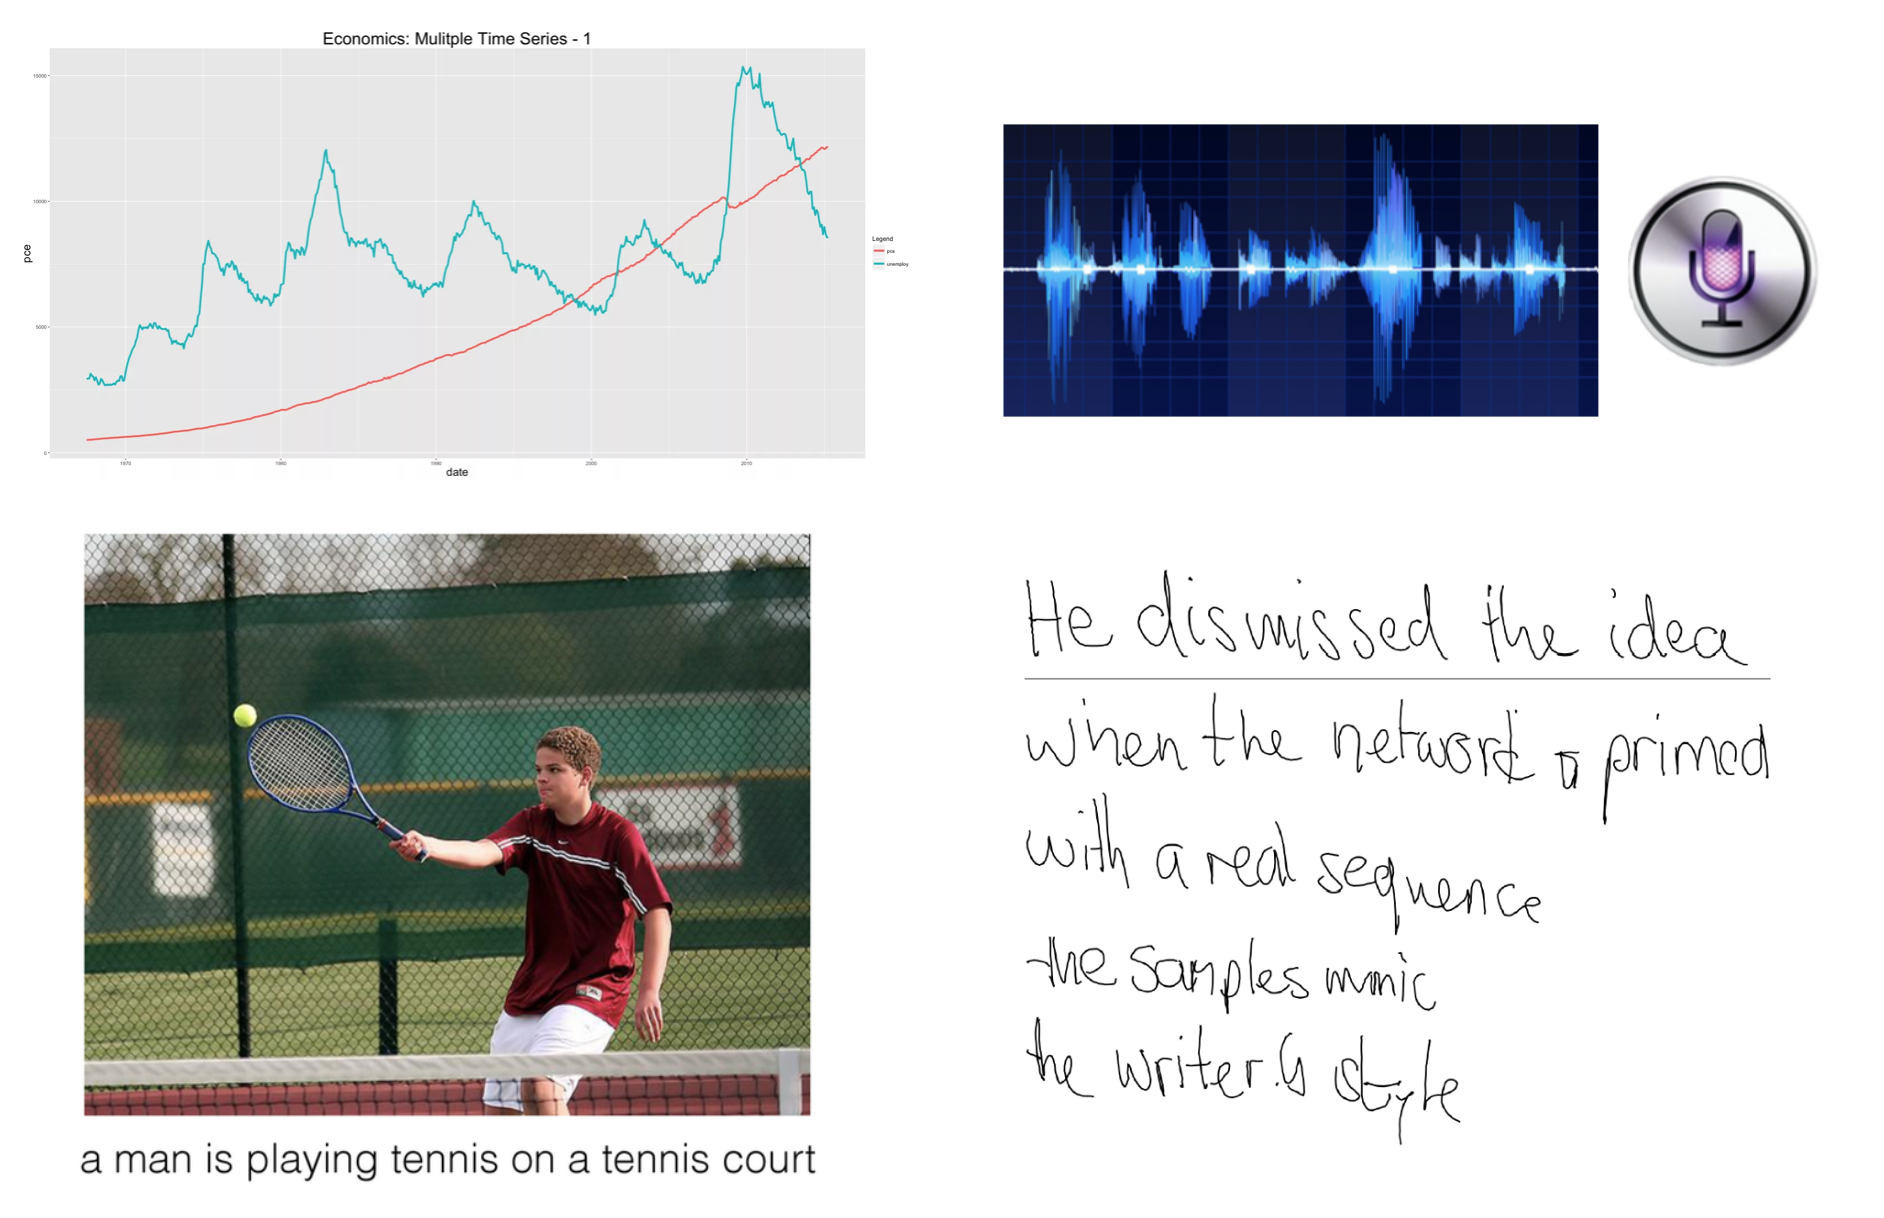
\includegraphics[width=.8\linewidth]{posled.png}
\end{center}
\end{frame}

\begin{frame}{Реуррентные сети}
\begin{center}
	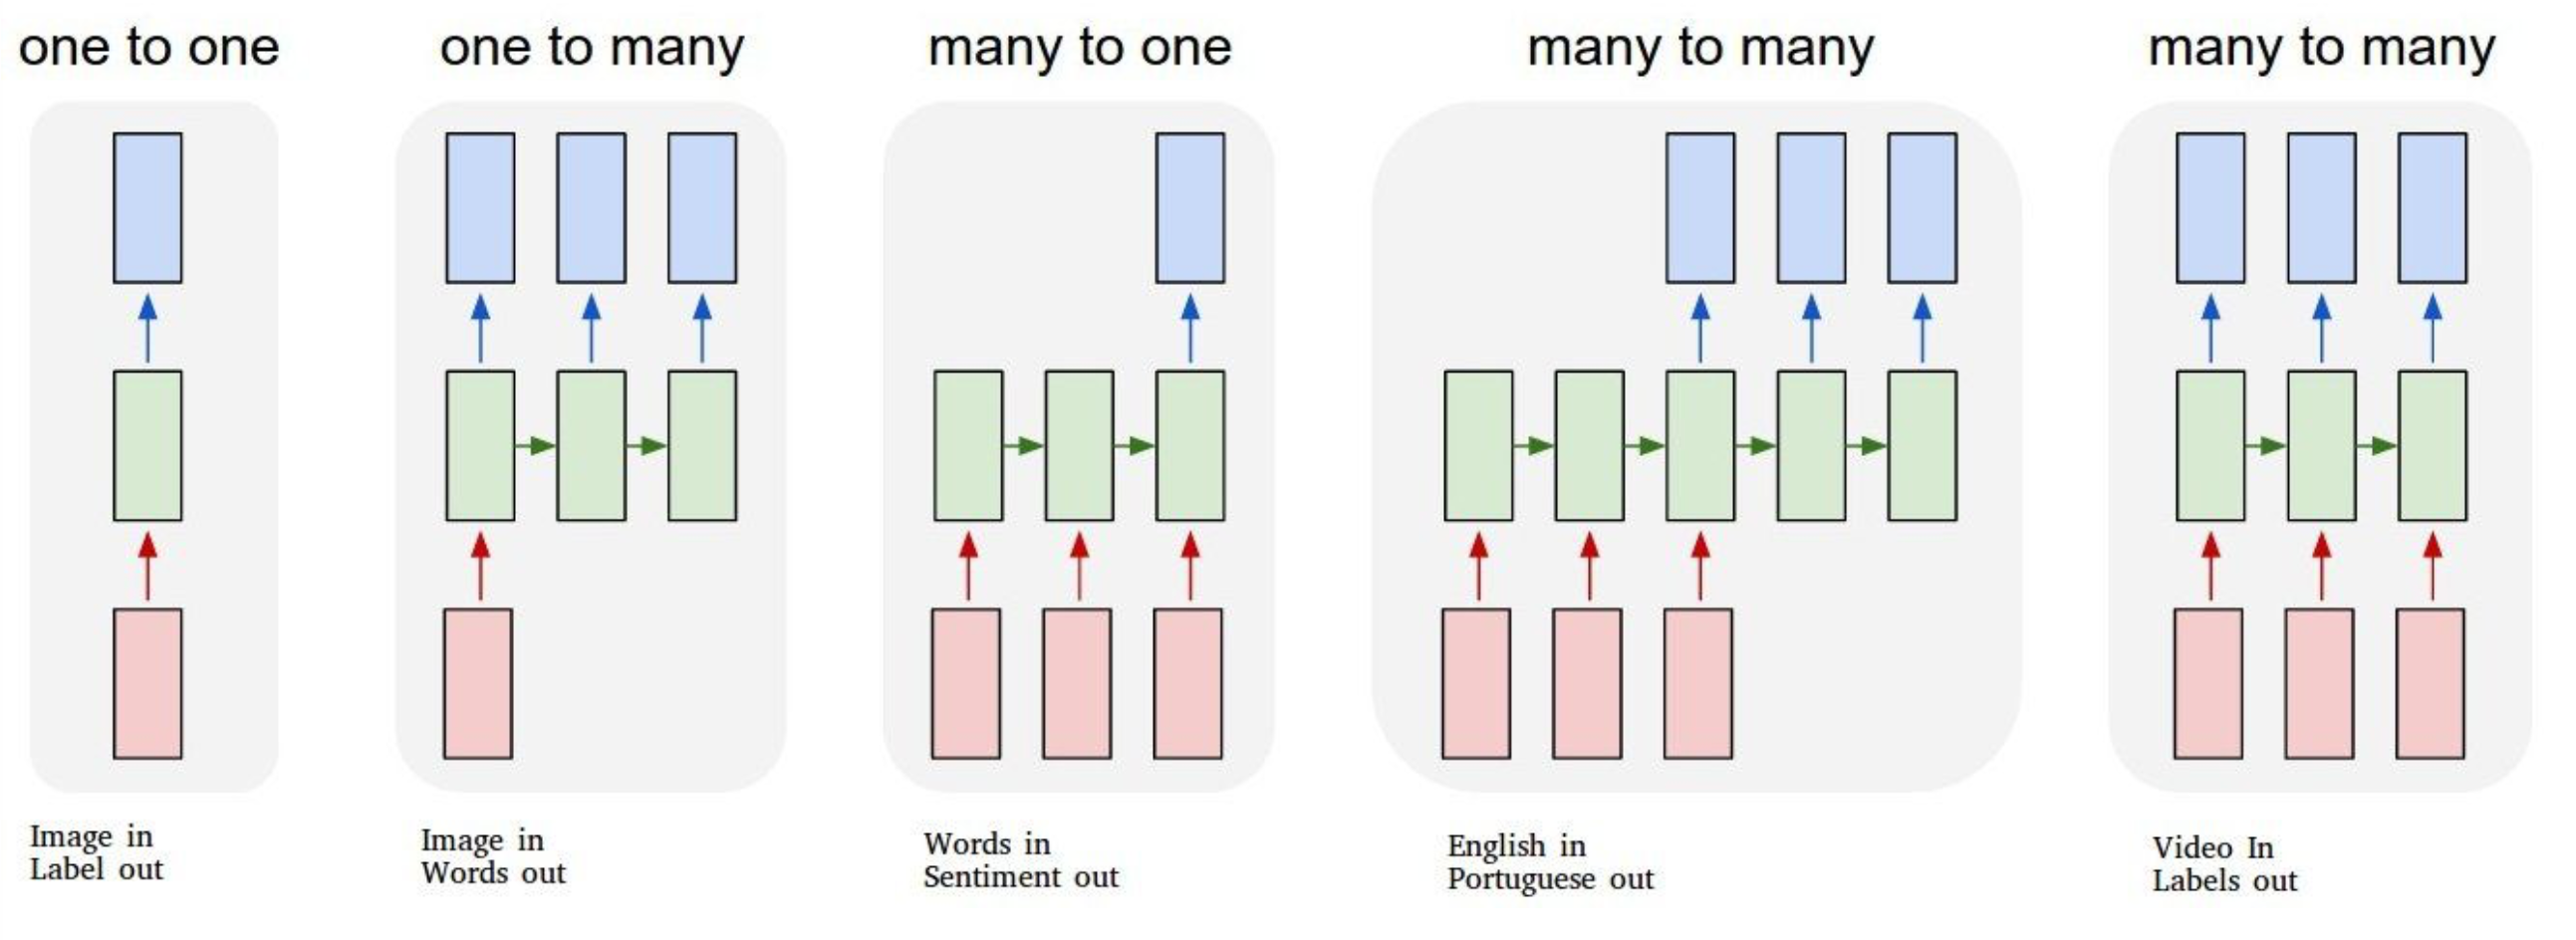
\includegraphics[width=.95\linewidth]{rnn_variants.png}
\end{center}
\end{frame}

\begin{frame}{Рекурентная сеть}
\begin{wideitemize} 
	\item  Каждый нейрон взаимодействует сам с собой 
	\item  На вход поступает последовательность (текст, видео, картинка, временной ряд), один и тот же нейрон просматривает её
	\item Впоследствие можно использовать эту сетку для генерации новых последовательностей (текстов, видео и тп)
\end{wideitemize} 
\end{frame}

\begin{frame}{От регрессии к нейрону}
\begin{center}
	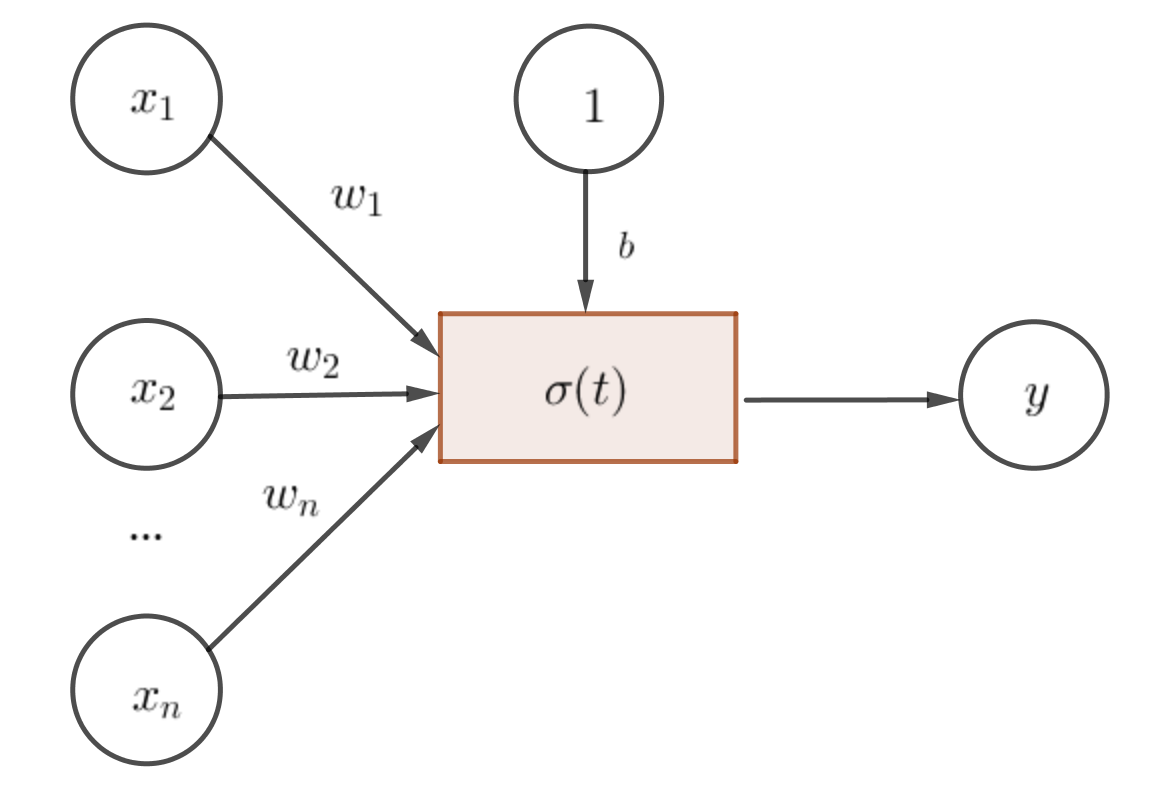
\includegraphics[width=.4\linewidth]{neuron_3.png}
\end{center}
\begin{equation*} 
	\begin{aligned}
		y_i =& b + w \cdot x_i \\
		&\Downarrow \\
		h_i =& b + w \cdot x_i \\
		y_i = & f(h_i)
	\end{aligned}
\end{equation*} 
\end{frame}


\begin{frame}{От авторегрессии к нейрону}
\begin{columns}	
	\begin{column}{.68\linewidth}
		\begin{equation*} 
		y_t = b + w \cdot y_{t-1} 
		\end{equation*} 
	\end{column}
	\begin{column}{.28\linewidth}
	\begin{center}
		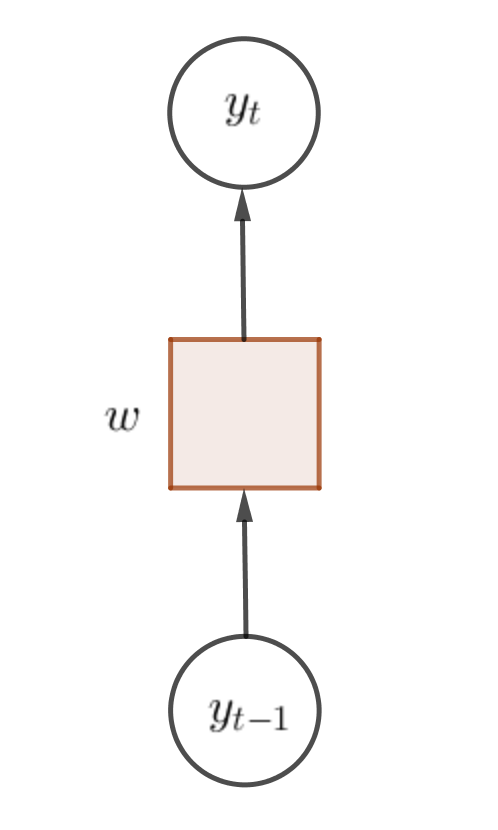
\includegraphics[width=.9\linewidth]{rec_neuron_1.png}
	\end{center}
\end{column}
\end{columns}
\end{frame}


\begin{frame}{От авторегрессии к нейрону}
\begin{columns}
	\begin{column}{.68\linewidth}
		\begin{equation*} 
		\begin{aligned}
		y_t =& b + w \cdot y_{t-1}\\
		&\Downarrow \\
	   h_t =& f_h(b_h + w \cdot h_{t-1} + v \cdot y_{t-1})\\
	   y_t =& f_y(b_y + u \cdot h_t)
		\end{aligned}
		\end{equation*} 
	\end{column}
	\begin{column}{.28\linewidth}
	\begin{center}
		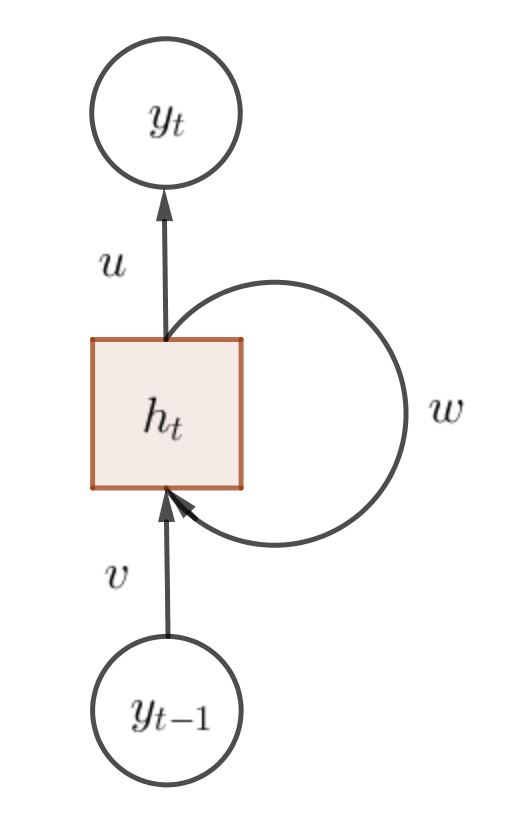
\includegraphics[width=.9\linewidth]{rec_neuron_2.png}
	\end{center}
\end{column}	
\end{columns}
\end{frame}


\begin{frame}{От авторегрессии к нейрону}
\begin{columns}
	\begin{column}{.68\linewidth}
		\begin{equation*} 
		\begin{aligned}
		h_t =& f_h(b_h + w \cdot h_{t-1} + v \cdot x_t)\\
		y_t =& f_y(b_y + u \cdot h_t)
		\end{aligned}
		\end{equation*} 
	\end{column}
	\begin{column}{.28\linewidth}
		\begin{center}
			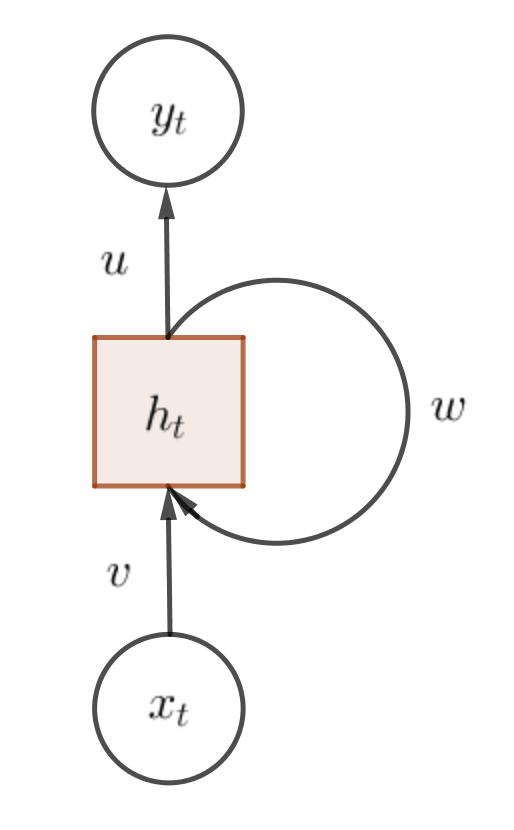
\includegraphics[width=.9\linewidth]{rec_neuron_3.png}
		\end{center}
	\end{column}	
\end{columns}
\end{frame}


\begin{frame}{Рекурентная сеть}
\begin{center}
	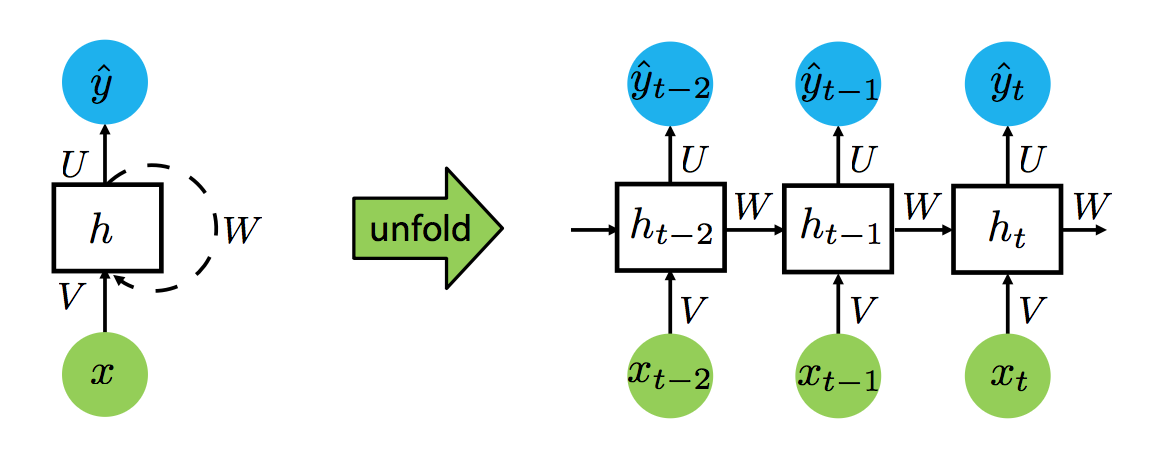
\includegraphics[width=.75\linewidth]{rnn.png}
\end{center}
\[
h_t = f_h( V x_t + W h_{t-1} + b_h) \qquad \hat y_t = f_y ( U h_t + b_y)
\]
\end{frame}

% Сюда сделать слайд со страницы 236 Николенко про типы задач, которые реашаются RNN

% картинка со страницы 233 и коммент
% Рекуррентную сеть можно рассматривать, как несколько копий одной и той же сети, каждая из которых передает информацию последующей копии. 

\begin{frame}{Рекурентная сеть}
\begin{wideitemize} 
	\item  \alert{Проблема} состоит в том, что в работе сетки появилось \alert{новое измерение: время} 
	
	\item На каждом шаге сетка взвешивает свой предыдущий опыт и новую информацию, получается, что при обучении, мы должны брать производную назад во времени
\end{wideitemize} 
\end{frame}


\begin{frame}{Рекурентная сеть}
\begin{columns}
	\begin{column}{.48\linewidth}
		\begin{wideitemize} 
			\item $y_t$ — настоящее значение
			\item $\hat{y_t}$  — прогноз
			\item $L_t(y_t, \hat{y_t})$  функция потерь
			\item $L = \sum_{t} L_t $
		\end{wideitemize} 
	\end{column}
	\begin{column}{.48\linewidth}
		\begin{center}
			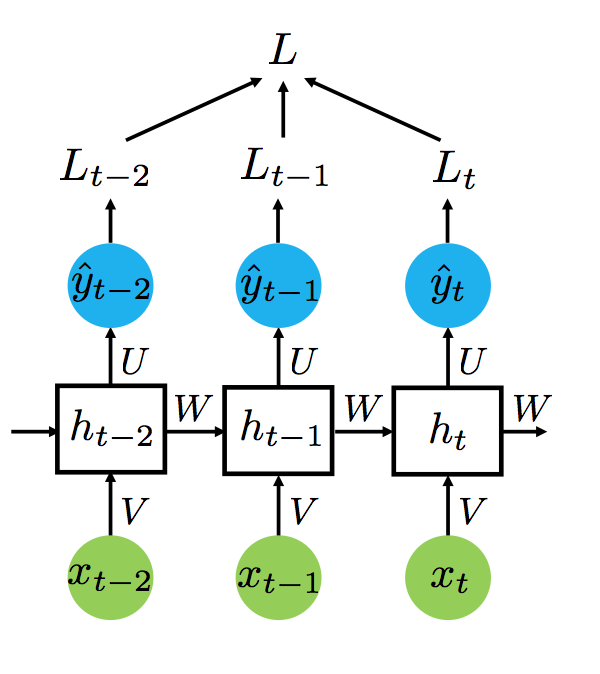
\includegraphics[width=.99\linewidth]{rnn0.png}
		\end{center}
	\end{column}	
\end{columns}
\end{frame}


\begin{frame}
\begin{center}
	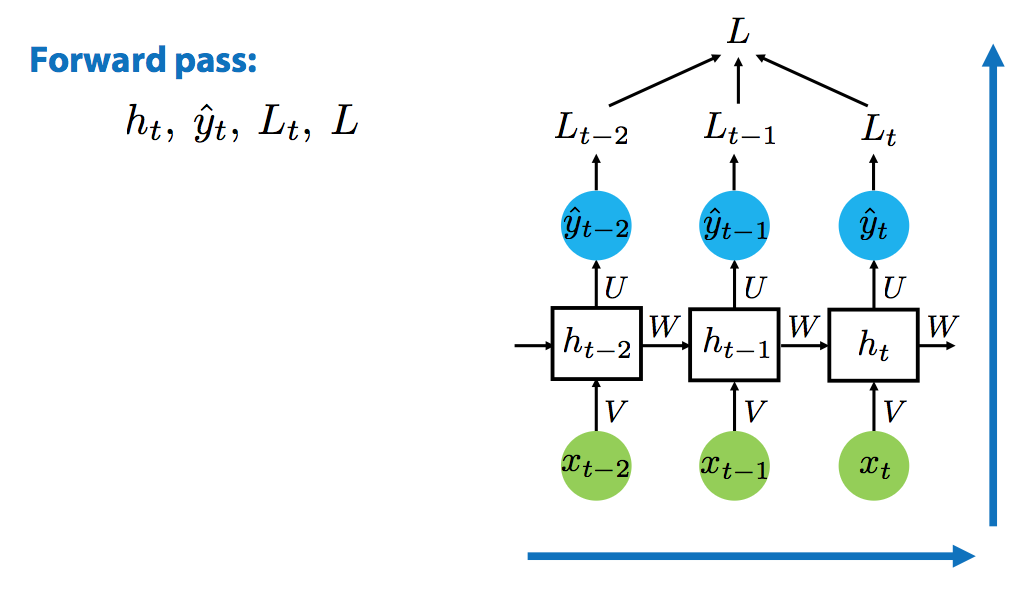
\includegraphics[width=.9\linewidth]{rnn2.png}
\end{center}
\end{frame}


\begin{frame}
\begin{center}
	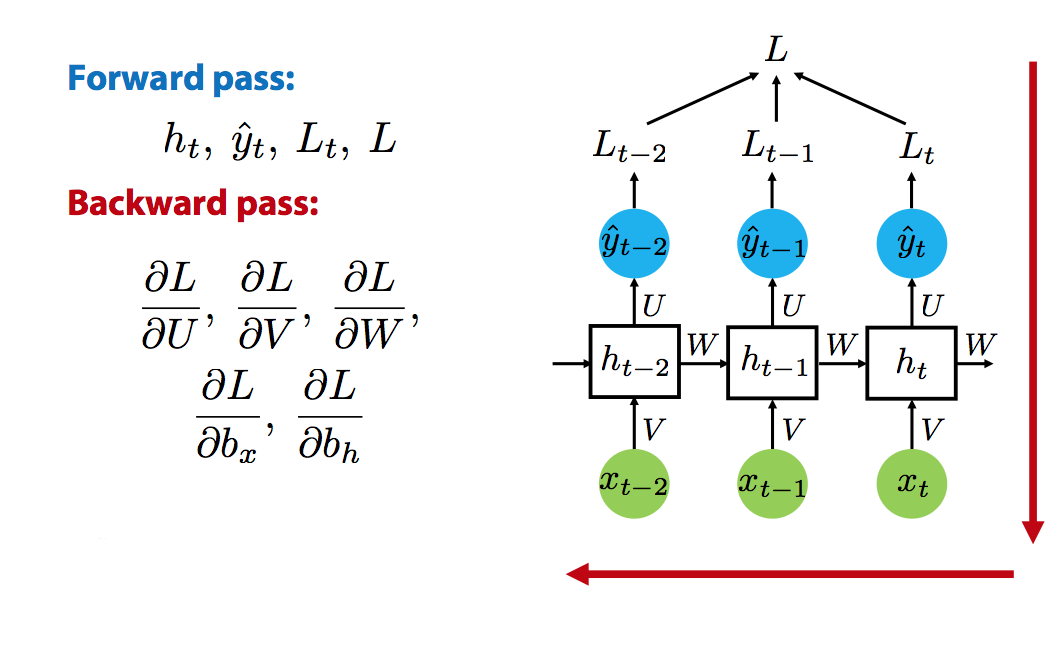
\includegraphics[width=.9\linewidth]{rnn3.png}
\end{center}
\end{frame}


\begin{frame}
\begin{center}
	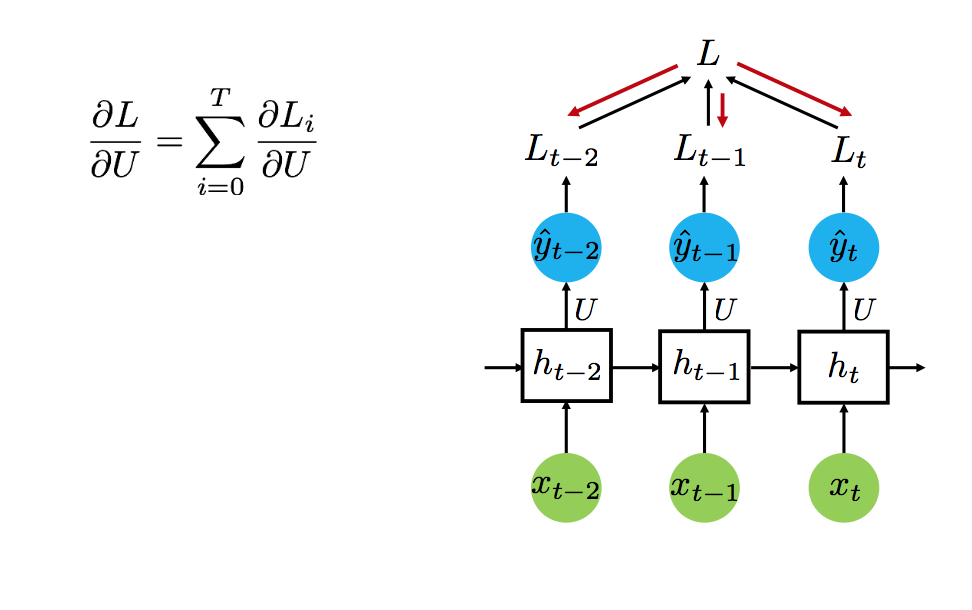
\includegraphics[width=.9\linewidth]{rnn4.png}
\end{center}
\end{frame}


\begin{frame}
\begin{center}
	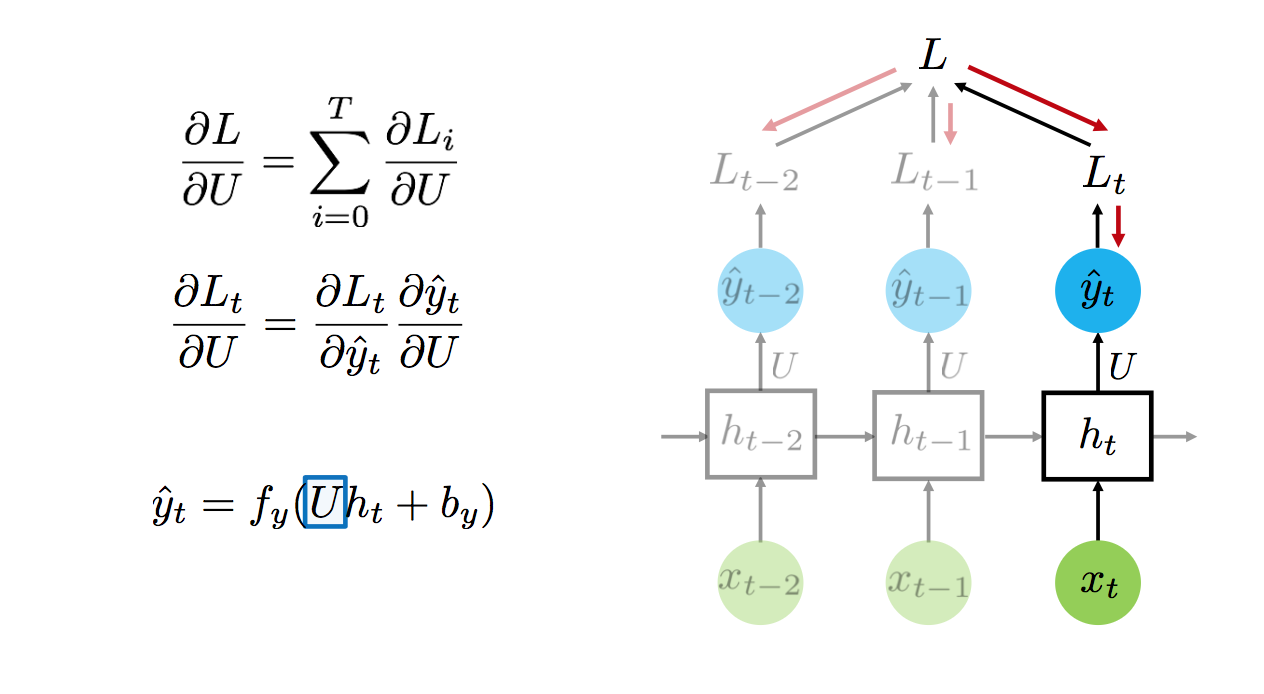
\includegraphics[width=.9\linewidth]{rnn5.png}
\end{center}
\end{frame}


\begin{frame}
\begin{center}
	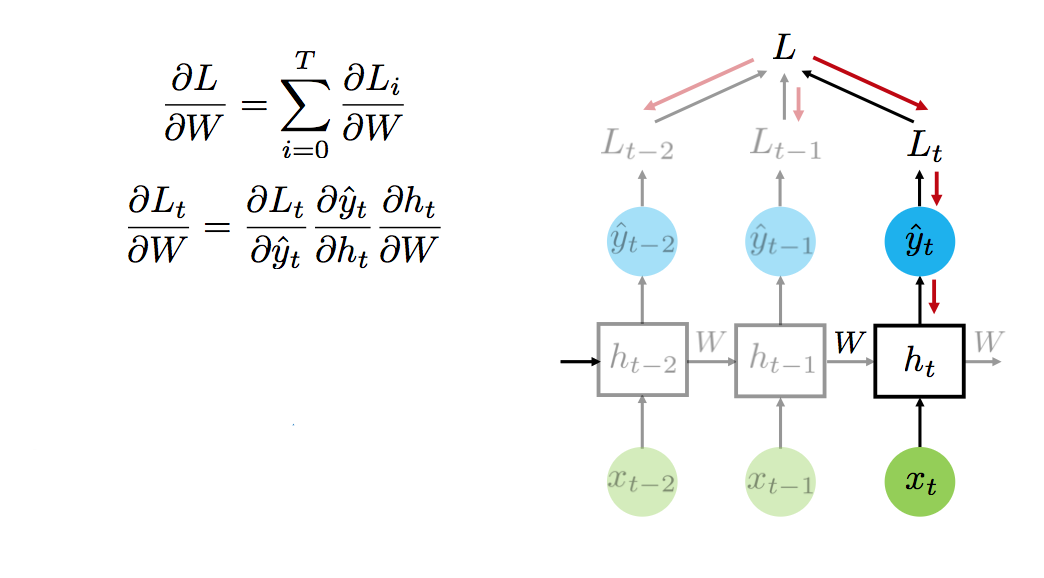
\includegraphics[width=.9\linewidth]{rnn6.png}
\end{center}
\end{frame}


\begin{frame}
\begin{center}
	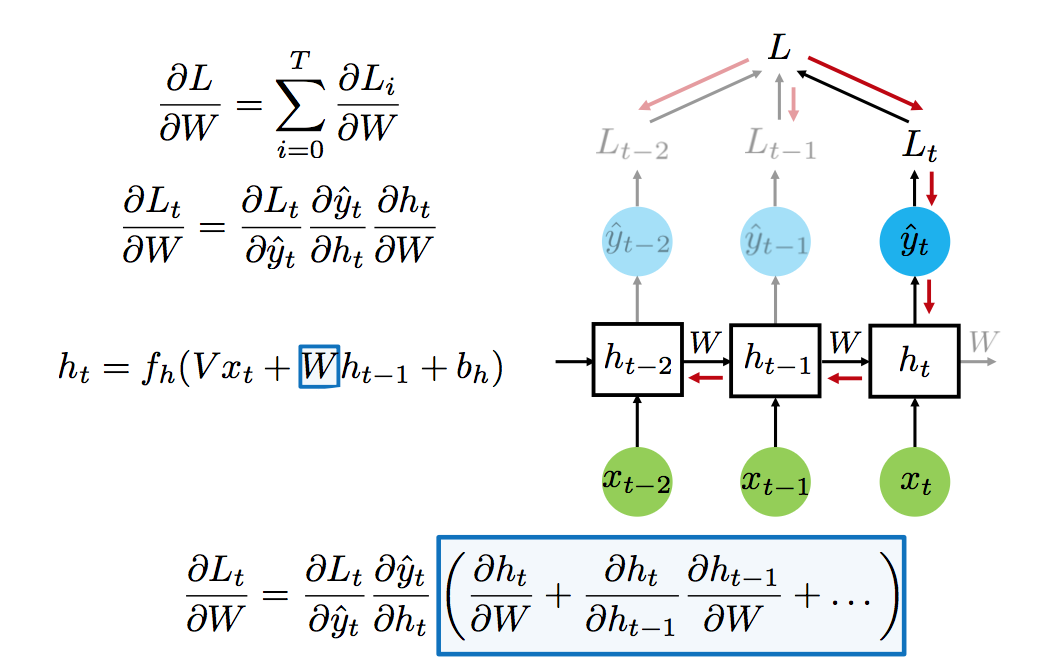
\includegraphics[width=.9\linewidth]{rnn7.png}
\end{center}
\end{frame}


\begin{frame}{Vanishing and Exploding}
\begin{center}
	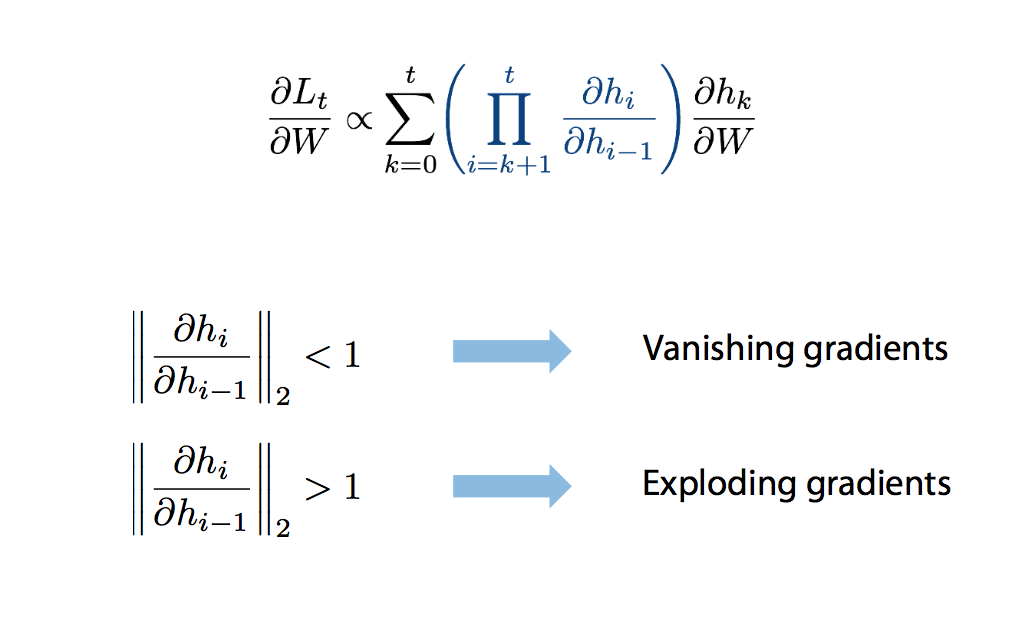
\includegraphics[width=.9\linewidth]{rnn8.png}
\end{center}
\end{frame}


\begin{frame}{Как понять, что градиент взорвался?}
\begin{center}
	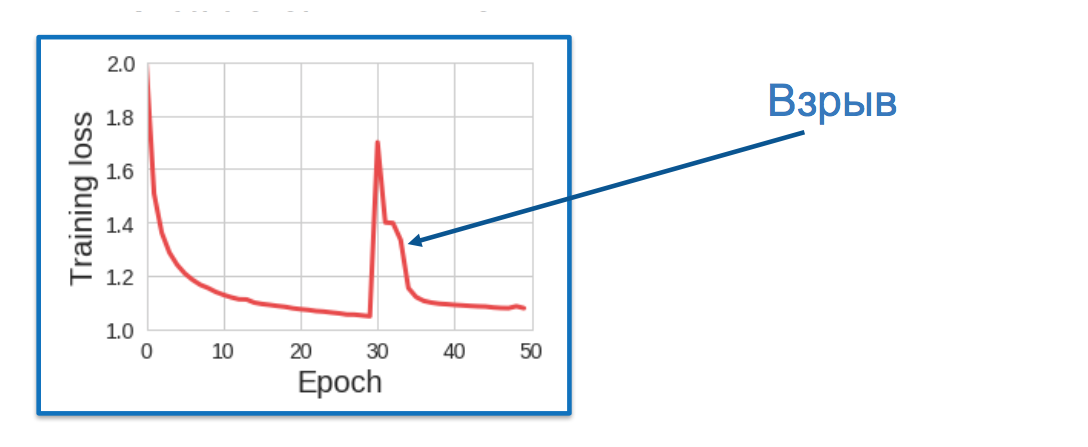
\includegraphics[width=.9\linewidth]{rnn9.png}
\end{center}
\end{frame}

\begin{frame}{Как предотвратить взрыв?}
\begin{wideitemize} 
\item Поставить порог, которые не будет пробиваться градиентом  (gradient clipping)

\item  Обучать сетку не целиком, а по кусочкам 

\item Аккуратно инициализировать веса

\item Делать skip-connection 

\item  Придумать специальную архитектуру 
\end{wideitemize} 
\end{frame}


\begin{frame}{Урезанное обучение}
\begin{center}
	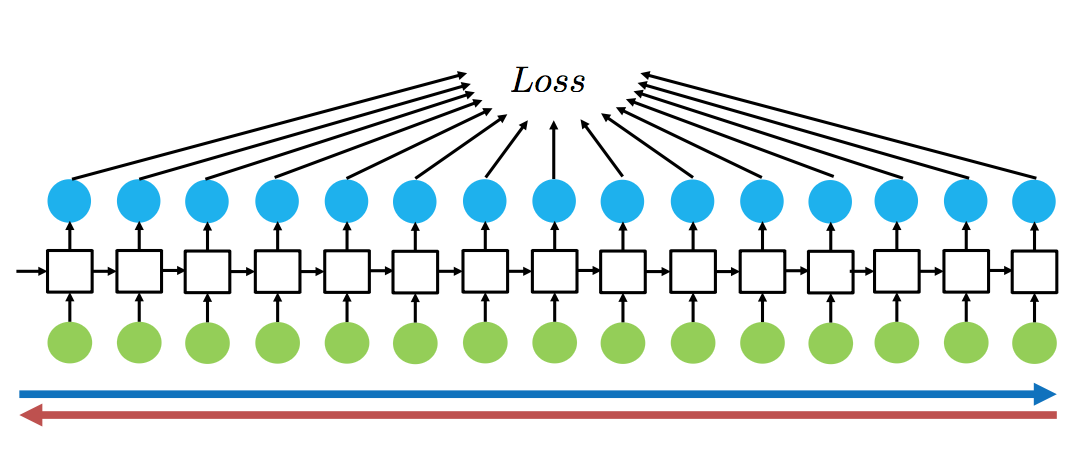
\includegraphics[width=.9\linewidth]{rnn10.png}
\end{center}
\end{frame}


\begin{frame}{Урезанное обучение}
\begin{center}
	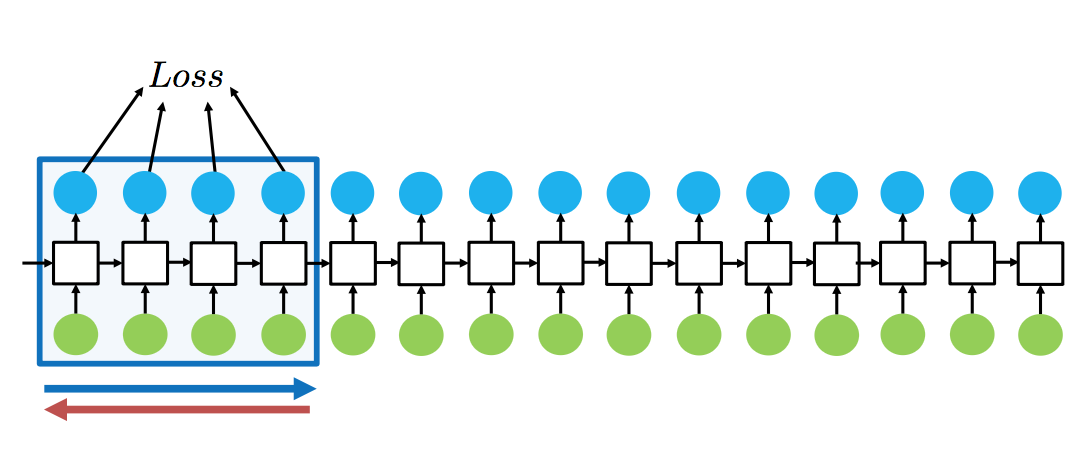
\includegraphics[width=.9\linewidth]{rnn11.png}
\end{center}
\end{frame}


\begin{frame}{Урезанное обучение}
\begin{center}
	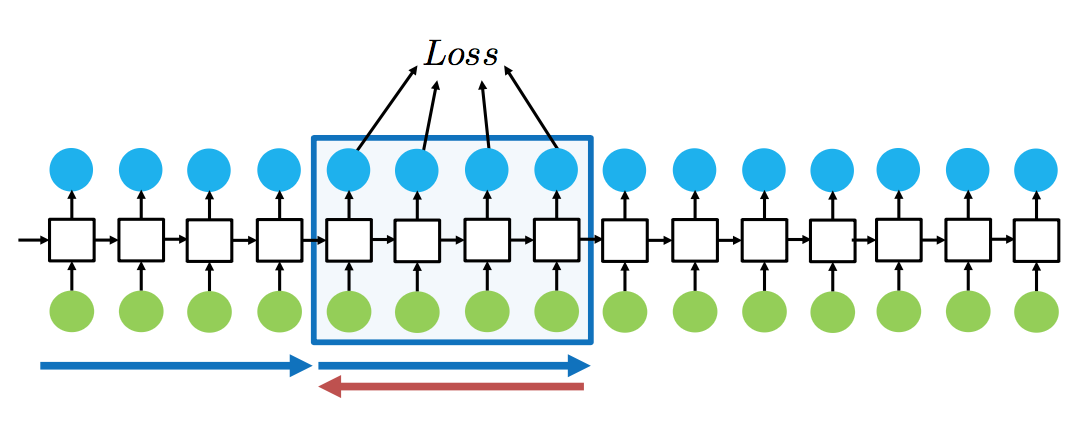
\includegraphics[width=.9\linewidth]{rnn12.png}
\end{center}
\end{frame}


\begin{frame}{Skip-connection}
\begin{center}
	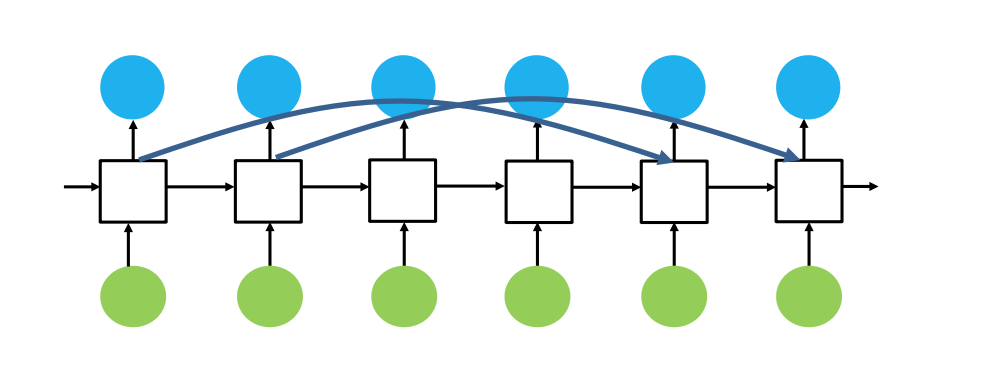
\includegraphics[width=.9\linewidth]{rnn13.png}
\end{center}
\end{frame}

\begin{transitionframe}
	\begin{center}
		\Huge LSTM (long short-term memory)
	\end{center}
\end{transitionframe}

\begin{frame}{Короткая память}
\begin{wideitemize}
	\item  Привлекательность RNN в том, что они потенциально умеют связывать предыдущую информацию с текущей
	
	\item При backpropagation текущие градиенты пробрасываются во времени назад
	
	\item  Если градиент не взрывается, он постепенно затухает, получается что влияние текущего слоя не может проброситься во времени слишком далеко назад 
	
	\item Влияние текущего слоя затухает экспоненциально по мере удаления и мешает обычным RNN находить в данных "далёкие" зависимости
\end{wideitemize}
\end{frame}


\begin{frame}{Короткая память}
\begin{center}
	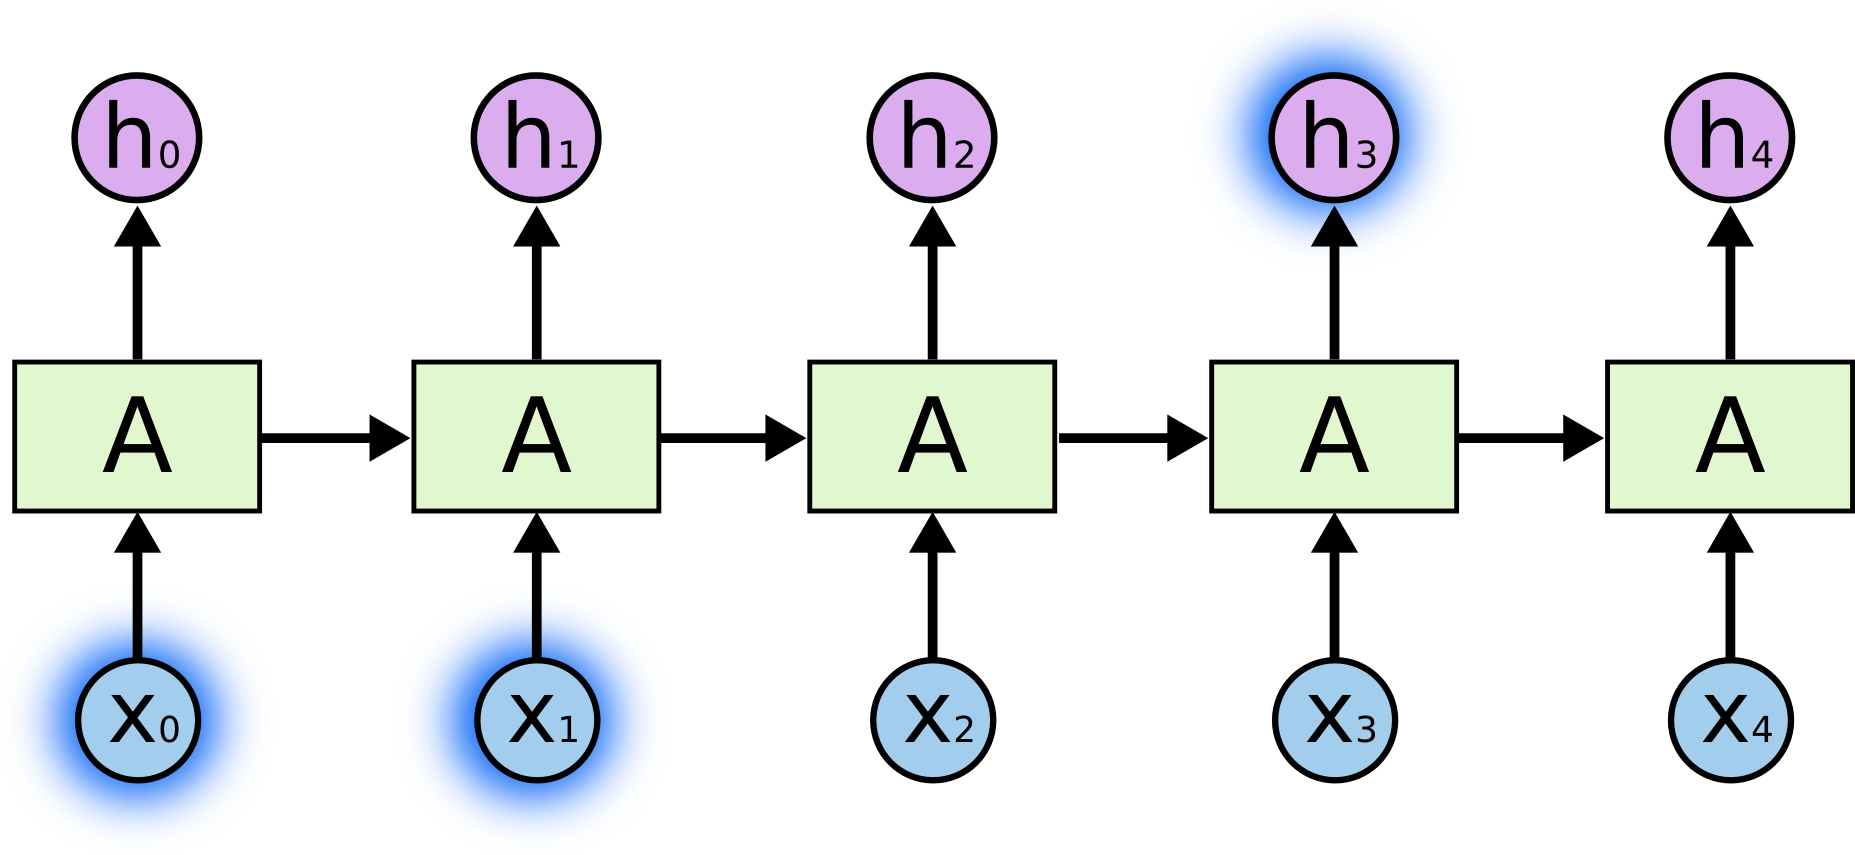
\includegraphics[width=.7\linewidth]{simple_rnn1.png}
\end{center}

\large Облака плывут по небу 
\end{frame}


\begin{frame}{Короткая память}
\begin{center}
	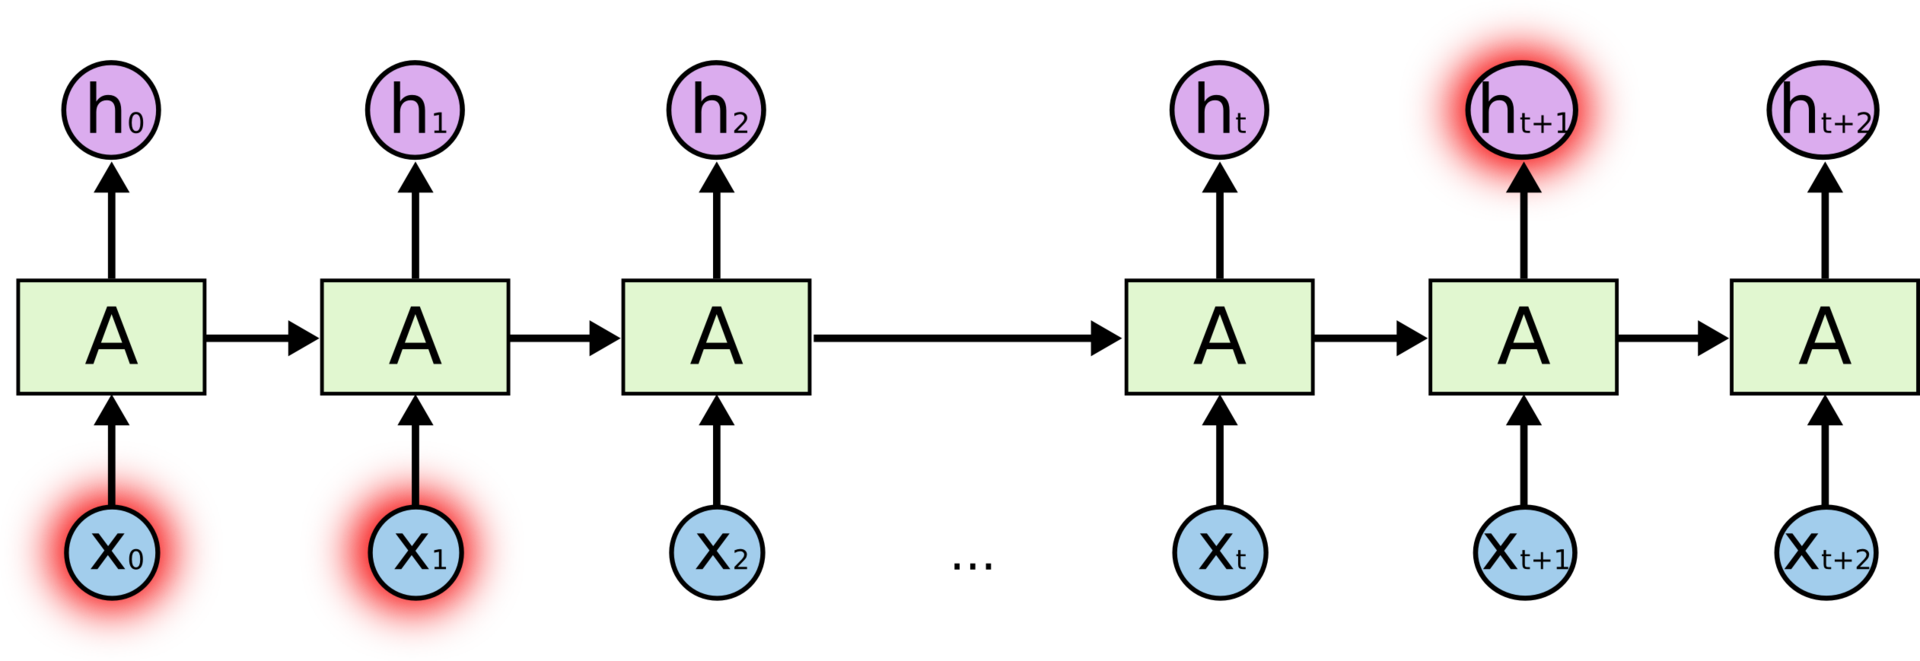
\includegraphics[width=.8\linewidth]{simple_rnn2.png}
\end{center}

\large Я вырос во Франции… Я бегло говорю по-французски
\end{frame}

\begin{frame}{Простейшая RNN}
\begin{center}
	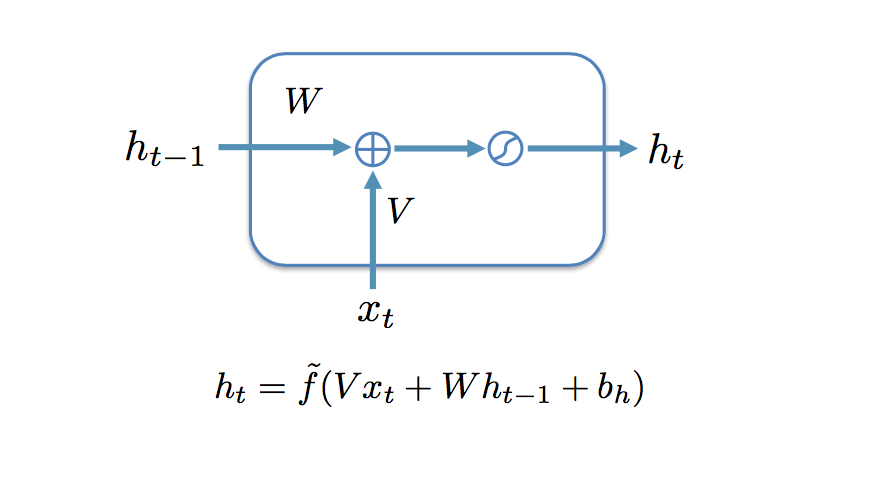
\includegraphics[width=.9\linewidth]{rnn14.png}
\end{center}
\end{frame}

\begin{frame}{Долгая краткосрочная память}
\begin{wideitemize}
	\item  Архитектура LSTM лечит эту проблему, она способна к обучению долговременным зависимостям.
	
	\item Внутри рекуррентной ячейки долгосрочная память моделируется явным образом. Конечно же нам из-за этого придётся учить больше параметров.
	
	\item Завораживающе! Так как же она выглядит?
\end{wideitemize}
\end{frame}


\begin{frame}{LSTM}
\begin{center}
	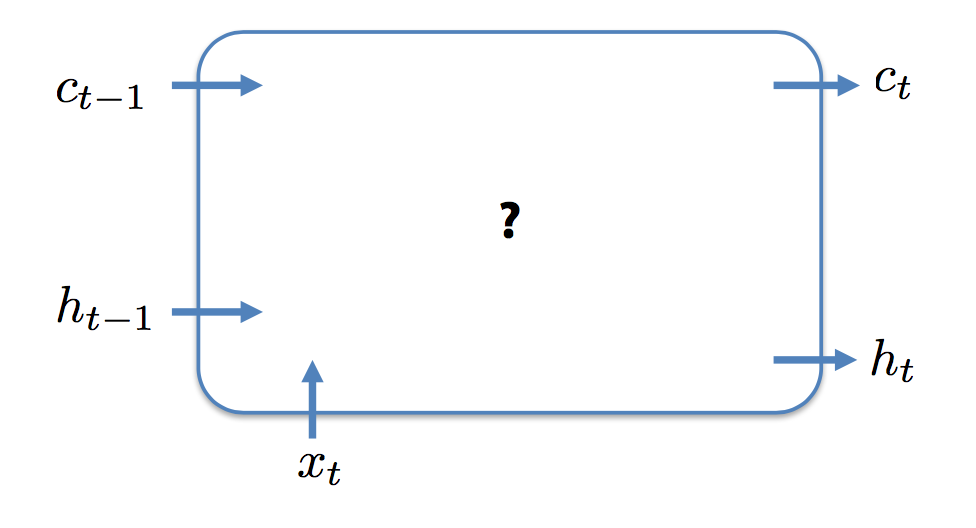
\includegraphics[width=.8\linewidth]{lstm1.png}
\end{center}
\end{frame}


\begin{frame}{LSTM}
\begin{center}
	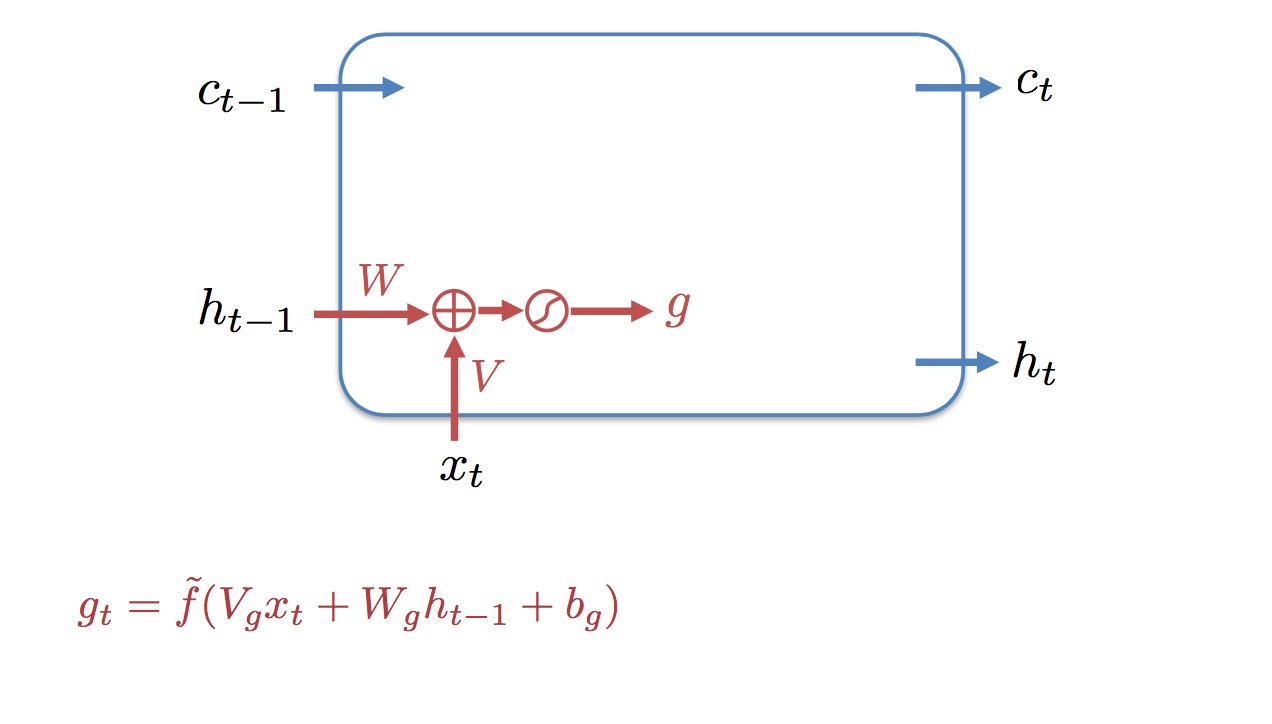
\includegraphics[width=.8\linewidth]{lstm2.png}
\end{center}
\end{frame}


\begin{frame}{LSTM}
\begin{center}
	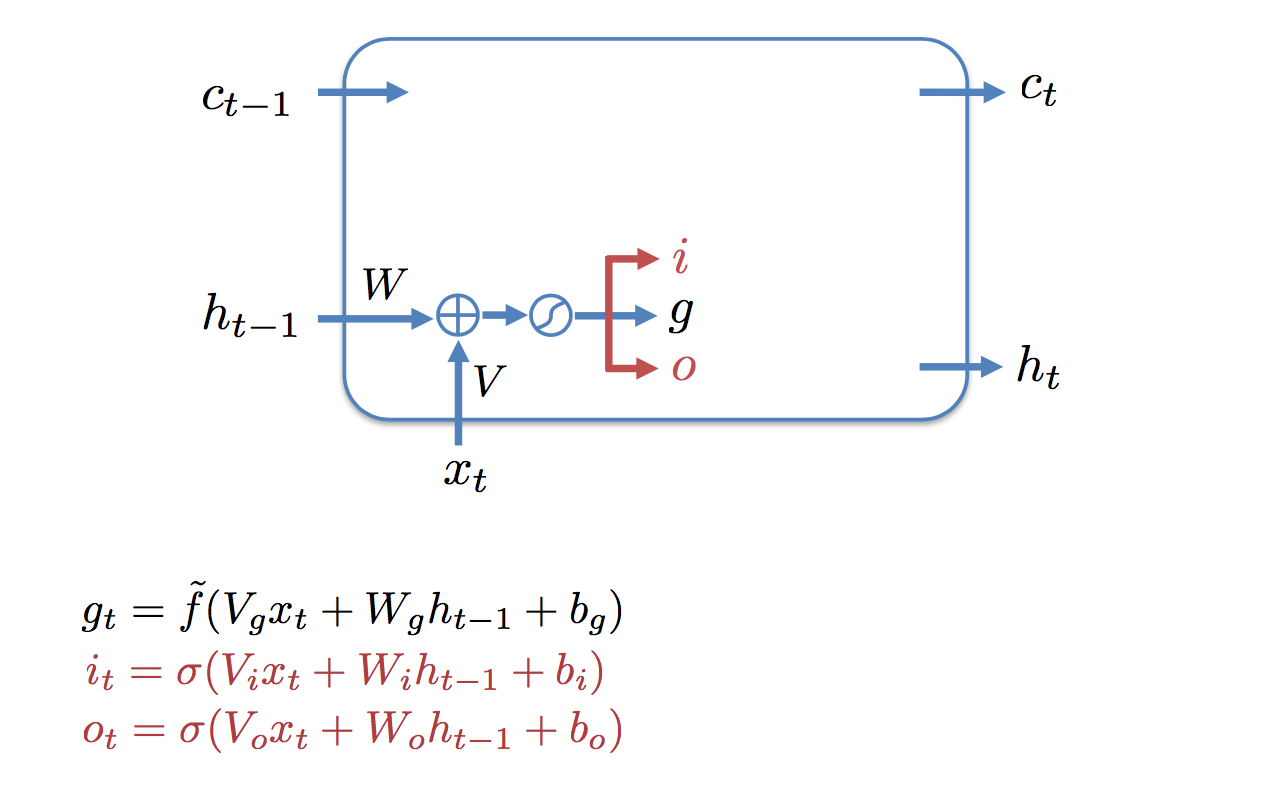
\includegraphics[width=.8\linewidth]{lstm3.png}
\end{center}
\end{frame}


\begin{frame}{LSTM}
\begin{center}
	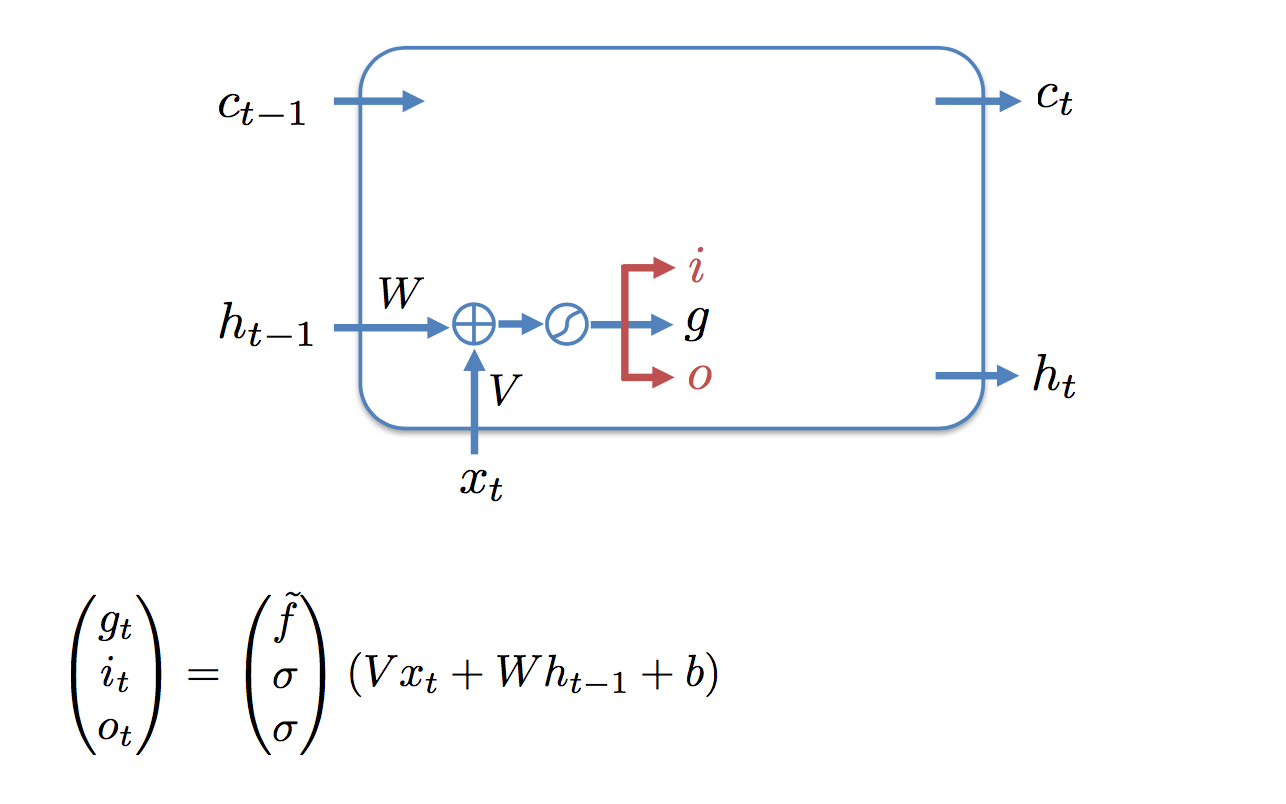
\includegraphics[width=.8\linewidth]{lstm4.png}
\end{center}
\end{frame}


\begin{frame}{LSTM}
\begin{center}
	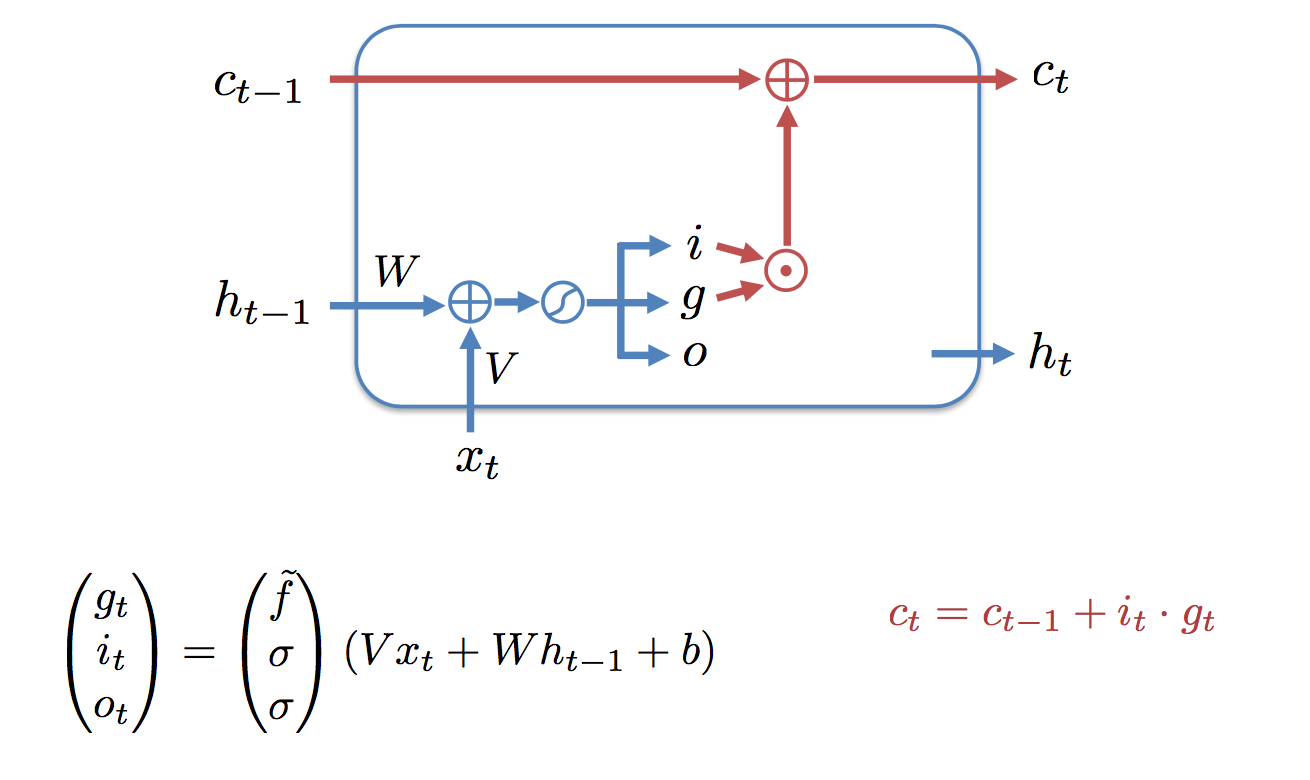
\includegraphics[width=.8\linewidth]{lstm5.png}
\end{center}
\end{frame}


\begin{frame}{LSTM}
\begin{center}
	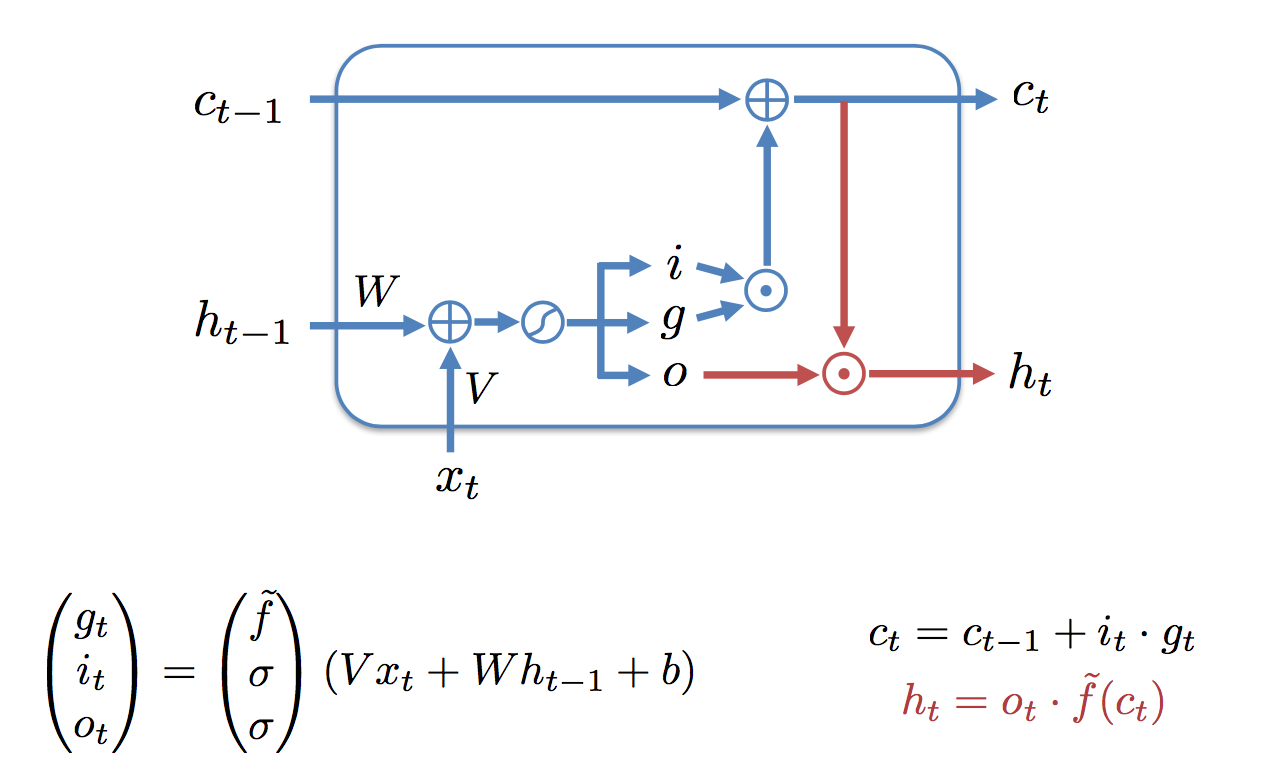
\includegraphics[width=.8\linewidth]{lstm6.png}
\end{center}
\end{frame}


\begin{frame}{LSTM}
\begin{wideitemize}
	\item  Ключевой элемент LSTM это состояние ячейки (cell state, $c_t$). Она проходит напрямую через цепочку, участвую лишь в нескольких линейных операциях. Информация может легко течь по ней не подвергаясь преобразованиям. 
	
	\item Фильтры (gates) контролируют поток информации и могут удалять лишнюю. Они состоят из слоя сигмоидальной нейронной сети и операции умножения. Сигмоида возвращает числа от $0$ до $1$, говоря какую долю информации нужно сохранить. 
	
	\item В LSTM три таких фильтра контролируют состояние ячейки. Часть забывается, часть берётся из нового входа. Все эти манипуляции делают ячейки очень гибкими. 
\end{wideitemize}
\end{frame}


\begin{frame}{LSTM}
\begin{center}
	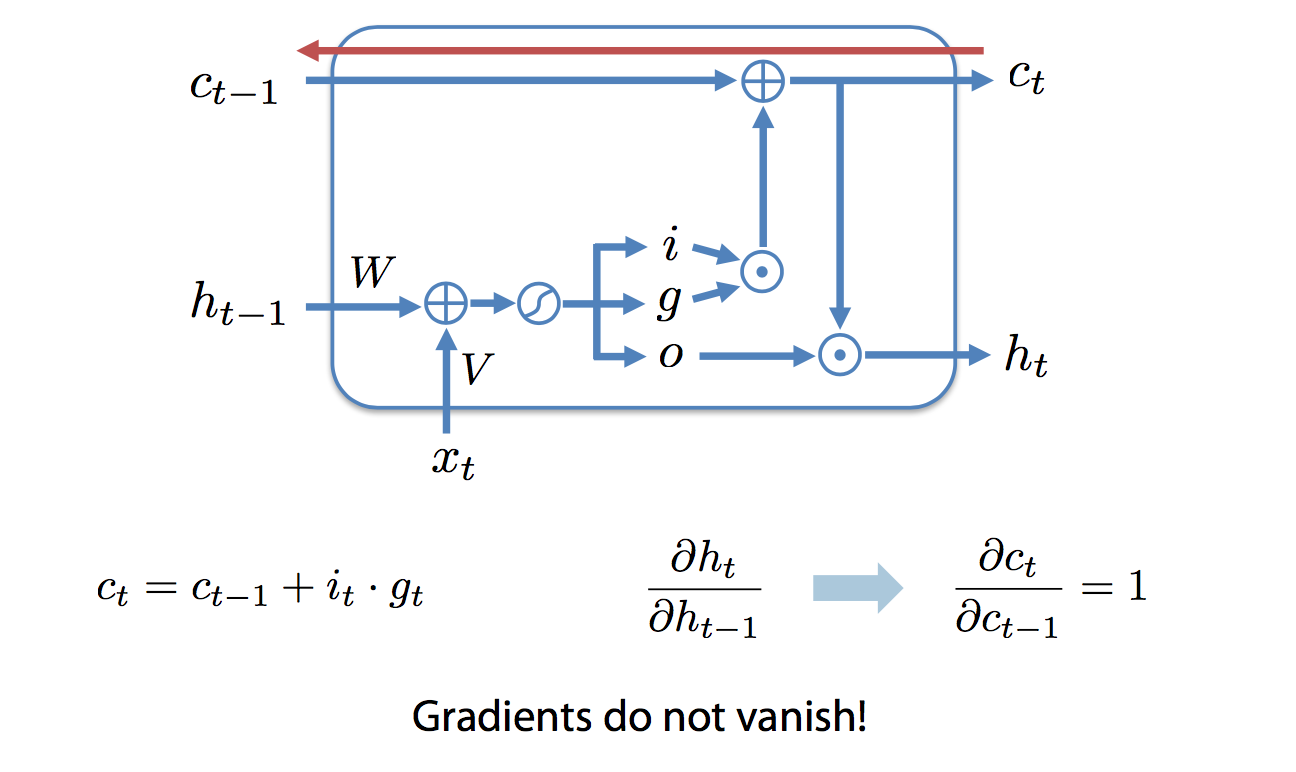
\includegraphics[width=.8\linewidth]{lstm7.png}
\end{center}
\end{frame}


\begin{frame}{LSTM}
\begin{wideitemize}
	\item  В рекурсивном вычислении состояния ячейки нет никакой нелинейности. Обычно это называют "каруселью константной ошибки". 
	
	\item Ошибка в LSTM пропагируется без изменений и скрытые состояния, если LSTM сама не решит их перезаписать, могут не меняться довольно долго.
	
	\item Такое устройство ячейки решает проблему исчезающих градиентов. Ошибка сама затухать не будет. Однако проблема взрывающихся градиентов остаётся. 
	
\end{wideitemize}
\end{frame}

\begin{frame}{LSTM c забыванием}
\begin{center}
	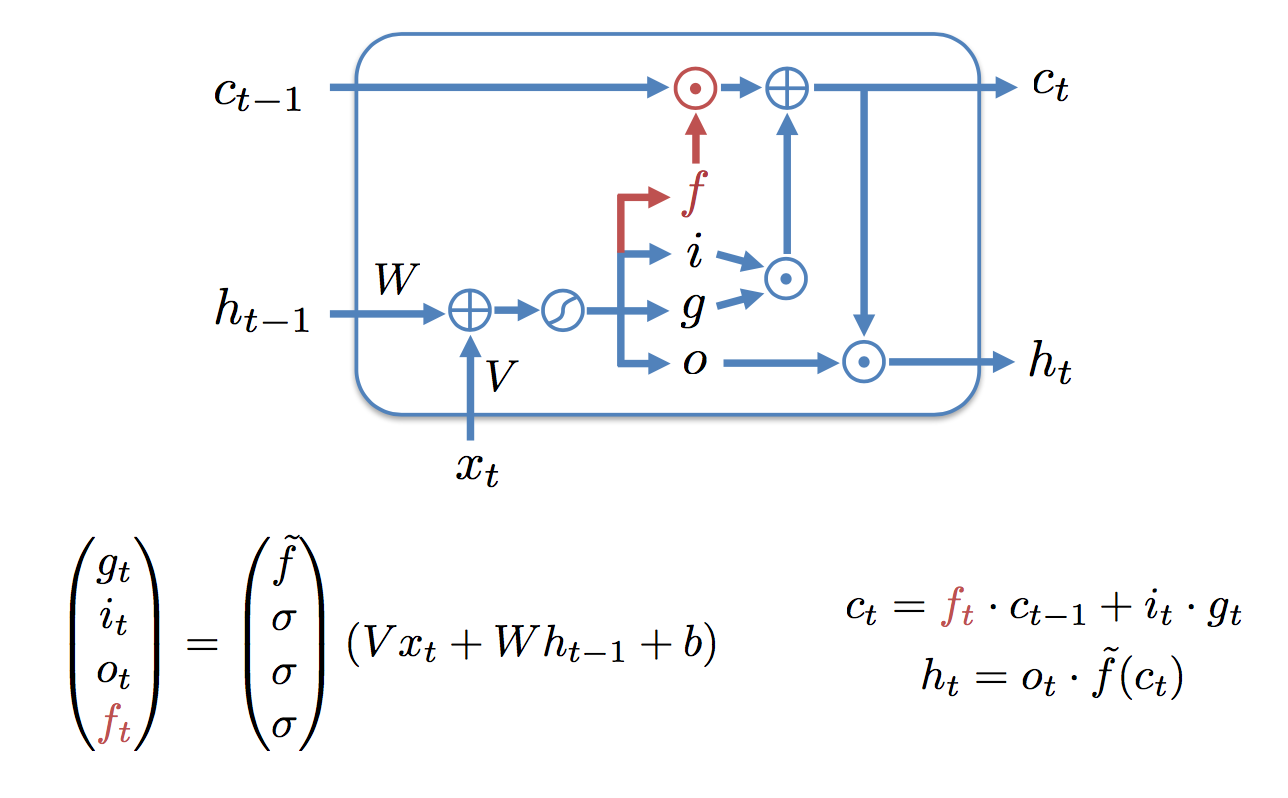
\includegraphics[width=.8\linewidth]{lstm8.png}
\end{center}
\end{frame}


\begin{frame}{LSTM c забыванием}
\begin{center}
	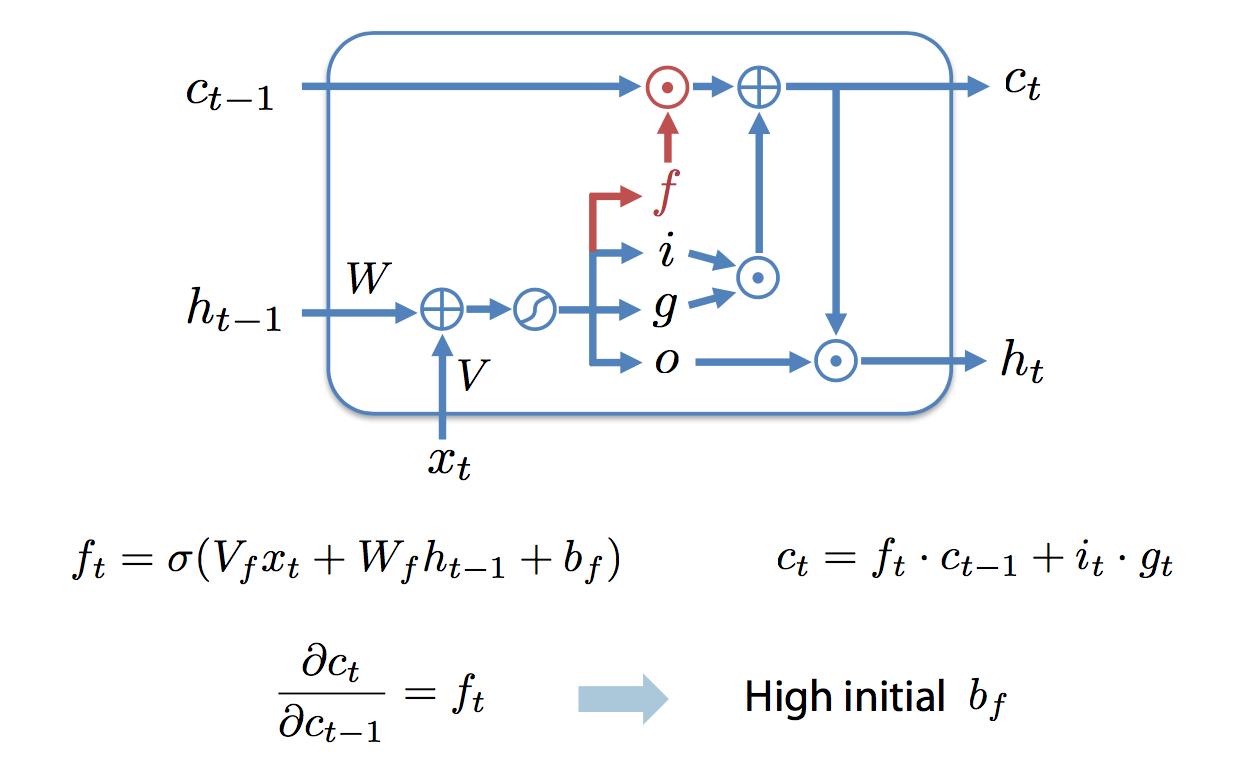
\includegraphics[width=.8\linewidth]{lstm9.png}
\end{center}
\end{frame}


\begin{frame}{А вот бы весов поменьше бы}
\begin{wideitemize}
	\item  В 2015 году придумали GRU-ячейку
	
	\item Придумали с желанием сохранить память в ячейке, но упростить LSTM
	
	\item Учиться и применяется на 20-50\% быстрее, результаты в большинстве случаев похожие
	
\end{wideitemize}
\end{frame}


\begin{frame}{GRU-ячейка}
\begin{center}
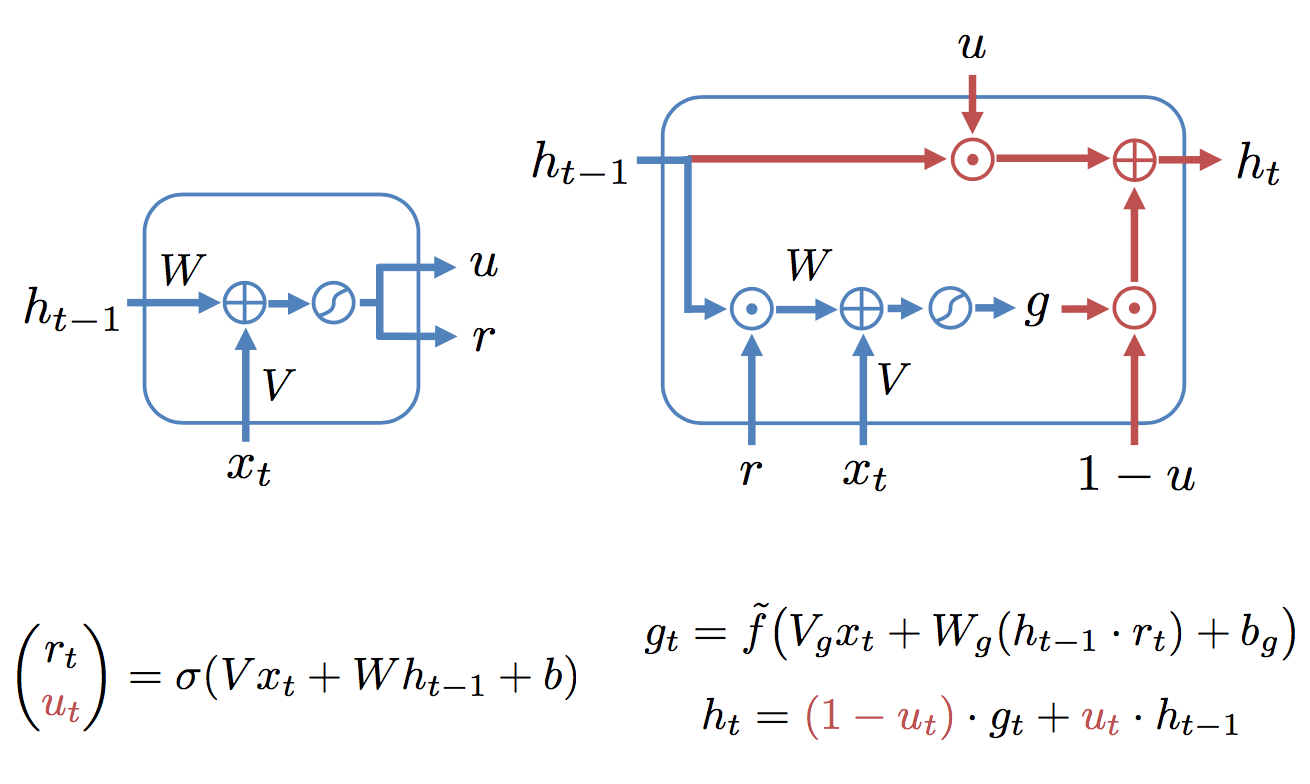
\includegraphics[width=.8\linewidth]{gry_1.png}
\end{center}
\end{frame}


\begin{frame}{Двунаправленные рекуррентные сети}
\begin{center}
	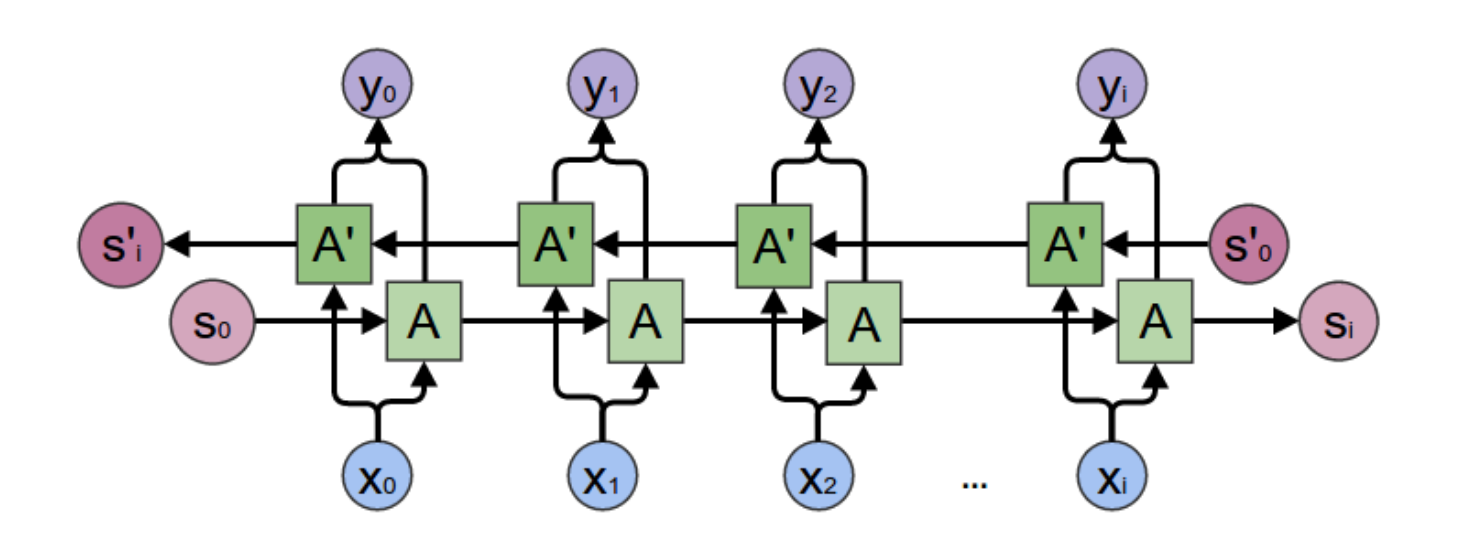
\includegraphics[width=.9\linewidth]{biderect_lstm.png}
\end{center}
\end{frame}


\begin{frame}{Двунаправленные рекуррентные сети}
\begin{wideitemize}
	\item  Часто RNN к концу последовательности забывает о том, с чего всё начиналось, последние элементы последовательности всегда будут важнее первых 
	
	\item Давайте один слой будет читать последовательность слева направо, а второй справа налево.  Разумеется это можно делать только для тех последовательностей, которые даны нам целиком (предложения, аудио)  и нельзя для тех, которые мы видим только в прошлое (валютный курс).
	
	\item Для каждого элемента получаем скрытое состояние, отражающее его контекст и слева и справа.
\end{wideitemize}
\end{frame}

\begin{transitionframe}
	\begin{center}
		\Huge Кросс-валидация для временных рядов 
	\end{center}
\end{transitionframe}

\begin{frame}{Cross validation on a rolling basis
}
\begin{center}
	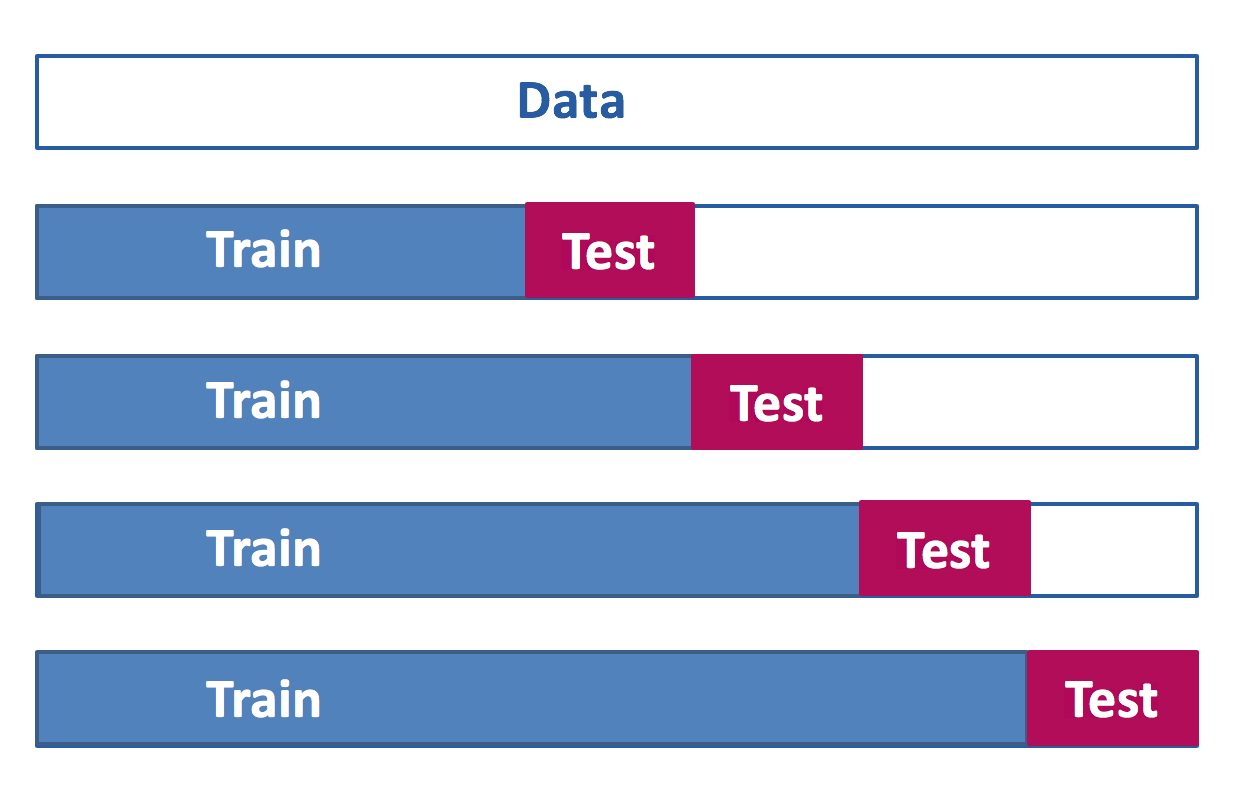
\includegraphics[width=.7\linewidth]{cv1.png}
\end{center}
\end{frame}


\begin{frame}{Cross validation on a rolling basis}
\begin{center}
	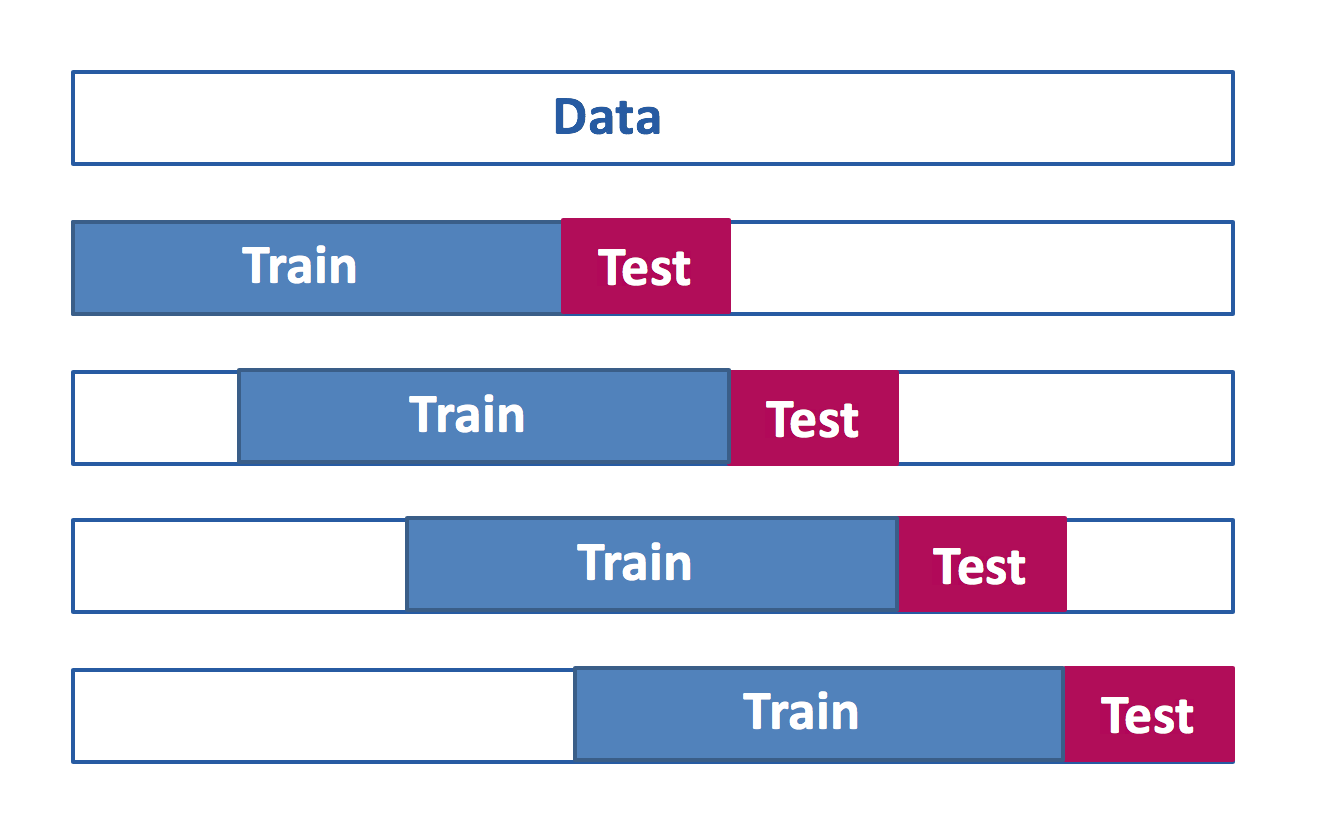
\includegraphics[width=.7\linewidth]{cv2.png}
\end{center}
\end{frame}


\begin{frame}{Cross validation on a rolling basis}
\begin{wideitemize}
	\item  \alert{Leave one out кросс-валидация} – когда в тест берём каждый раз только одно, следующее наблюдение

	
	\item Нельзя приравнивать разные горизонты прогнозирования 

	
	\item Модель может хорошо прогнозировать на неделю вперёд, но при этом плохо прогнозировать на месяц вперёд, либо наоборот 
	
	\item Иногда метрики вычисляют для разных горизонтов прогнозирования отдельно
\end{wideitemize}
\end{frame}



\end{document}
